\documentclass[a4paper,fleqn]{cas-dc}

\usepackage[numbers,sort&compress]{natbib}
\usepackage{graphicx}
\usepackage{float}
\usepackage{algorithm}
\usepackage{algpseudocode}
\usepackage{amsmath,amssymb}
\usepackage{booktabs}
\usepackage{multirow}
\usepackage{makecell}
\usepackage{pifont}

\newcommand{\cmark}{\ding{51}}
\newcommand{\xmark}{\ding{55}}
\newcommand{\gain}[1]{\ensuremath{(+#1)}}
% Suppress the empty ORCID footnote printed by the CAS template.
\RenewDocumentCommand{\printorcid}{}{}

\begin{document}
\let\WriteBookmarks\relax
\renewcommand\floatpagefraction{.85}
\renewcommand\dblfloatpagefraction{.85}
\renewcommand\textfraction{.05}

\shorttitle{PAMA-SDD++}
\shortauthors{Long et~al.}

\title[mode=title]{PAMA-SDD++: Reliability-Aware Pyramid-Agent Mediation for Scale-Decoupled Knowledge Distillation}

\author[1]{Shiyu Long}
\cormark[1]
% Add the full e-mail address before submission.
% \ead{your.email@example.com}

\affiliation[1]{organization={Nanjing University of Aeronautics and Astronautics},
    city={Nanjing},
    postcode={210016},
    country={China}}

\cortext[cor1]{Corresponding author.}

\begin{abstract}
Knowledge distillation is an effective route to compact visual recognition,
but the usual image-level supervision compresses a teacher's decision into a
single probability vector and hides the spatial evidence that produced it.
Scale-decoupled distillation (SDD) exposes this evidence by matching local
logits over multi-scale grids. Its strength, however, is also its weakness:
regular partitions often contain incomplete object parts, mixed foreground and
background, or low-confidence teacher predictions, and independent local
matching can fragment the semantics that the teacher represents globally. This
paper treats SDD as a problem of \emph{reliability-aware local--global semantic
mediation} rather than independent grid supervision. The resulting framework,
PAMA-SDD++, keeps the teacher frozen and uses only stable teacher targets:
global logits, classifier-induced local logits, and non-parametric agent
relations. On the student side, Progressive Semantic Pyramid Calibration
(PSPC) forms a semantically calibrated pyramid before region partition, while
Cross-Scale Agent Mediation (CSAM) condenses multi-scale evidence into compact
agents that return global context to local regions and provide an
architecture-agnostic relation interface for distillation. The optimization
couples three constraints: reliability-aware local distillation suppresses
uncertain partitions, Local--Global Coherence ties each local prediction to
the teacher's image-level belief, and relation-graph Global Agent Consistency
aligns the organization among agents instead of raw feature channels. Across
CIFAR-100, ImageNet-1K, and CUB-200-2011, PAMA-SDD++ improves KD-, DKD-, and
NKD-based SDD baselines, with the largest gains on fine-grained recognition.
All mediation modules are used only during training, so the deployed student
keeps the original inference cost. Code will be released at
\textcolor{blue}{https://github.com/Cherxy/PAMA-SDD}.
\end{abstract}

% Use if graphical abstract is present
% \begin{graphicalabstract}
% \includegraphics{figs/grabs.pdf}
% \end{graphicalabstract}

% Research highlights
% \begin{highlights}
% \item Research highlights item 1
% \item Research highlights item 2
% \item Research highlights item 3
% \end{highlights}

% Keywords
% Each keyword is separated by \sep
\begin{keywords}
Knowledge distillation \sep 
Scale-decoupled distillation \sep 
Reliability-aware local distillation \sep
Cross-scale agent mediation \sep 
Fine-grained image classification
\end{keywords}


\maketitle



\section{Introduction}

The accuracy of modern image classifiers has grown together with model
capacity, yet many recognition systems must still run under tight memory,
latency, and energy budgets~\cite{tan2021efficientnetv2,mehta2022mobilevit,
liu2022convnext}. Knowledge distillation (KD) addresses this gap by training
a compact \emph{student} with guidance from a high-capacity
\emph{teacher}~\cite{hinton2015distilling,gou2021knowledge,wang2020kdreview}.
The teacher can provide softened output distributions, intermediate features,
or relational structures that are absent from one-hot labels. In image
classification, such supervision is especially attractive because it improves
the deployed model without changing the inference architecture.

\begin{figure}[pos=t]
	\centering
	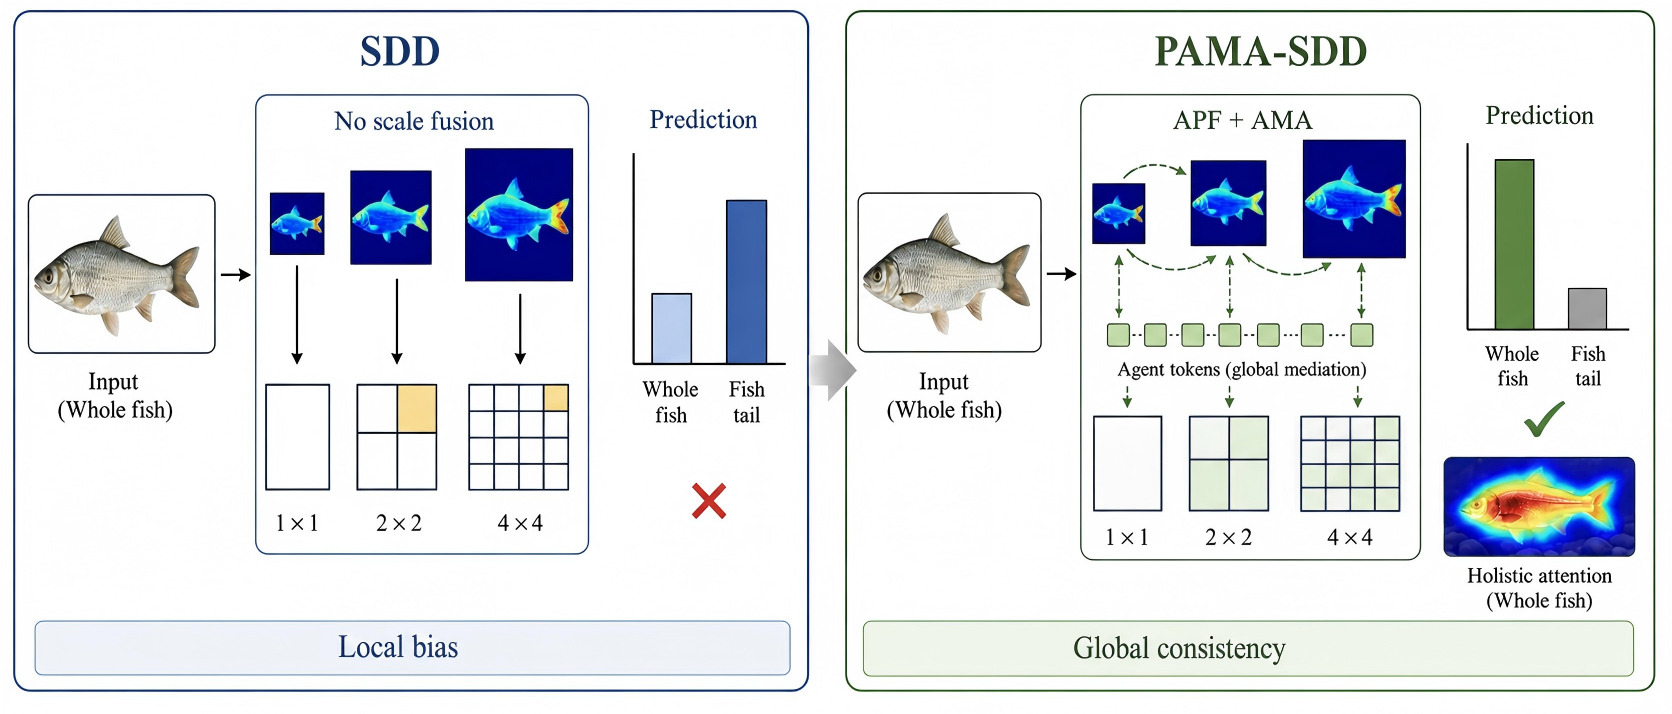
\includegraphics[width=\linewidth]{figs/motivation_refined.png}
	\caption{
		Motivation of PAMA-SDD++. SDD exposes local classification evidence by
		partitioning features into regular grids, but a grid cell can contain
		incomplete object parts, background-biased regions, or uncertain teacher
		predictions. PAMA-SDD++ filters local targets by reliability and
		mediates them through pyramid-agent global semantics.
	}
	\label{fig:motivation}
\end{figure}

Most classification KD methods can be read as different answers to one
question: what form of teacher knowledge should the student inherit?
Logit-based methods align output distributions and are simple to apply across
heterogeneous architectures~\cite{hinton2015distilling,zhao2022decoupled,
yang2023knowledge}. Feature-based methods transfer intermediate activations,
attention maps, or transformed responses~\cite{romero2015fitnets,
zagoruyko2017paying,chen2021distilling,touvron2021deit}. Relation-based and
contrastive methods preserve sample-wise or structural organization in the
teacher representation space~\cite{tung2019similarity,park2019relational,
tian2020contrastive,xu2020selfsupervision}. These signals are powerful, but
many of them are produced after global spatial aggregation. The student learns
which classes the teacher prefers, but only weakly observes where the evidence
for that preference lies.

The missing spatial evidence matters when recognition depends on parts,
textures, or object structure, as in fine-grained
classification~\cite{zhuang2020apinet,du2020pmg,rao2021counterfactual,
he2022transfg}. Scale-Decoupled Distillation (SDD) makes this evidence
explicit by partitioning a feature map into multi-scale grids and distilling
local logits for the resulting regions~\cite{wei2024scaled}. This simple idea
brings the teacher closer to the visual evidence used by the student. It also
creates a new problem. A regular grid cell is not a semantic object: it may cut
through the foreground, contain background clutter, or isolate a weak local
cue. Matching every local prediction with the same confidence can therefore
amplify unreliable targets. Moreover, local logits trained in isolation can
become confident on fragments while drifting away from the teacher's
image-level belief. More local supervision is not automatically better; the
local evidence must be judged by reliability and tied back to global semantics.

This paper follows that observation to a single premise:
scale-decoupled distillation should be formulated as
\emph{reliability-aware local--global semantic mediation}. A practical method
should satisfy three conditions. First, it should prepare a coherent
multi-scale student representation before producing local logits. Second, it
should reduce the influence of uncertain teacher regions without discarding
hard local cases. Third, it should connect local student predictions with the
teacher's global decision and semantic organization. These requirements lead
to \textbf{PAMA-SDD++}, a pyramid-agent framework for classification-oriented
SDD.

PAMA-SDD++ keeps the teacher fixed and uses stable targets from the teacher's
global logits, classifier-induced local logits, and non-parametric pooled
agent relations. All trainable mediation happens on the student side. First,
Progressive Semantic Pyramid Calibration (PSPC) propagates deep semantic
context to higher-resolution student features through a channel--spatial
adaptive gate. Second, Cross-Scale Agent Mediation (CSAM) summarizes the
calibrated pyramid with a small set of agents, lets those agents gather
regional evidence, and broadcasts the resulting global context back to local
tokens. Third, the training objective combines reliability-aware local
distillation, Local--Global Coherence (LGC), and relation-graph Global Agent
Consistency (GAC). These losses respectively suppress uncertain grid targets,
bind local predictions to the teacher's image-level distribution, and transfer
agent-level semantic structure without requiring channel-wise feature matching.
The teacher, PSPC, CSAM, local logits, and all auxiliary losses are removed at
test time; deployment uses the original student network.

The contributions are:
\begin{itemize}
    \item \textbf{A local--global mediation formulation for SDD.} We identify
    unreliable partitions and weak local--global consistency as two central
    limitations of grid-based local distillation, and recast SDD as
    reliability-aware semantic mediation rather than independent grid matching.

    \item \textbf{A stable pyramid-agent distillation framework.} PAMA-SDD++
    combines frozen, well-defined teacher targets with student-side PSPC and
    CSAM modules, producing calibrated multi-scale local evidence and compact
    agent-level global context during training.

    \item \textbf{A coupled reliability and relation objective.} The proposed
    loss couples reliability-aware local distillation, LGC, and relation-graph
    GAC, allowing the student to inherit local evidence, global teacher belief,
    and agent semantic organization in one optimization objective.

    \item \textbf{Evidence across scales and tasks.} Experiments on CIFAR-100,
    ImageNet-1K, and CUB-200-2011 show consistent improvements over KD-, DKD-,
    and NKD-based SDD baselines. Ablations and visual analysis support the
    roles of pyramid calibration, agent mediation, local reliability, and
    relation-graph consistency, with no added inference cost.
\end{itemize}

\section{Related Work}
\label{sec:related_work}

\subsection{Knowledge Distillation}
\label{subsec:kd}

Knowledge distillation has developed from response matching into a broad
family of teacher--student training strategies~\cite{hinton2015distilling,
gou2021knowledge,wang2020kdreview}. Response-based methods transfer softened
class probabilities and remain attractive because they are architecture
agnostic. Recent logit objectives such as DKD~\cite{zhao2022decoupled} and
NKD~\cite{yang2023knowledge} further refine the target and non-target class
signals. Feature-based methods provide more direct representation guidance
through intermediate hints~\cite{romero2015fitnets,chen2021distilling},
attention maps~\cite{zagoruyko2017paying}, masked generation
targets~\cite{yang2022masked}, or cross-layer semantic
calibration~\cite{chen2021semckd,mirzadeh2020teacher,xu2020selfsupervision}.
Relation-based and contrastive approaches preserve inter-sample similarity,
relational geometry, or contrastive structure in the teacher representation
space~\cite{tung2019similarity,park2019relational,tian2020contrastive}.

PAMA-SDD++ is complementary to these objectives. It does not replace the base
logit loss; instead, KD, DKD, and NKD can all instantiate the global and local
distillation terms. The difference lies in the supervision geometry: the
student is not only matched to a global output or a dense feature map, but is
trained with reliability-weighted local predictions and agent-level global
semantic relations.

\subsection{Scale-Decoupled Distillation}
\label{subsec:sdd}

Conventional logit distillation compresses the image into a single prediction
vector~\cite{hinton2015distilling,zhao2022decoupled,yang2023knowledge}. This
global signal is efficient, but it can hide the parts and textures that drive
the teacher's decision, especially in fine-grained
recognition~\cite{zhuang2020apinet,du2020pmg,he2022transfg}.
Scale-Decoupled Distillation (SDD)~\cite{wei2024scaled} responds by producing
local logits from multi-scale grid partitions. The student therefore receives
explicit local supervision rather than only image-level class probabilities.

The open issue is that grid cells are not guaranteed to be reliable semantic
units. A local target can be useful, noisy, or globally inconsistent depending
on how the grid overlaps with the object. PAMA-SDD++ preserves SDD's local
logit interface while adding reliability estimation, local--global coherence,
and agent relation alignment. The local targets are therefore used as
evidence, not as equally trusted independent labels.

\subsection{Multi-Scale Feature Fusion}
\label{subsec:multiscale}

Multi-scale fusion is a standard way to reconcile high-level semantics with
low-level spatial detail~\cite{qiao2021detectors,wang2021pvt,
xie2021segformer}. FPN~\cite{lin2017feature} uses top-down lateral
connections, PANet~\cite{liu2018panet} adds bottom-up propagation,
BiFPN~\cite{tan2020efficientdet} learns efficient bidirectional weights, and
ASFF~\cite{liu2019asff} performs spatially adaptive fusion to reduce conflicts
between scales~\cite{qiao2021detectors,wang2021pvt,liu2021swin}. These
architectures mainly target recognition or detection accuracy by improving the
backbone representation.

PSPC adopts the same general insight but uses it in a different role. It is a
training-only calibration module for distillation: before local logits are
constructed, deep semantic context is propagated to higher-resolution student
features so that grid-level supervision is derived from a more coherent
multi-scale basis.

\subsection{Attention and Global Context Modeling}
\label{subsec:attention}

Attention mechanisms capture long-range dependencies in visual
representations~\cite{dosovitskiy2021vit,liu2021swin,bao2022beit,he2022mae}.
Self-attention in Transformers~\cite{vaswani2017attention} and non-local
operations in convolutional networks~\cite{wang2018nonlocal} model global
token interactions directly, but dense interaction is costly for
high-resolution feature maps~\cite{wang2021pvt,liu2021swin,dong2022cswin,
wu2021cvt}. Efficient attention variants reduce this cost through approximate
or mediated interactions~\cite{katharopoulos2020linear,choromanski2021performer}.
Agent Attention~\cite{han2024agent}, for example, uses a compact set of agent
tokens to gather information from image tokens and then broadcast it back.

CSAM follows the mediated-interaction principle but assigns the agents a
distillation-specific role. The agents are initialized from the calibrated
student pyramid, used to return global context to local regions, and then
compared with non-parametric teacher agents through relation graphs. This
turns attention from a representation enhancer into a compact interface for
cross-network semantic organization transfer.





\section{Methodology}
\label{sec:method}

\subsection{Overview of PAMA-SDD++}

\begin{figure*}[pos=t]
    \centering
    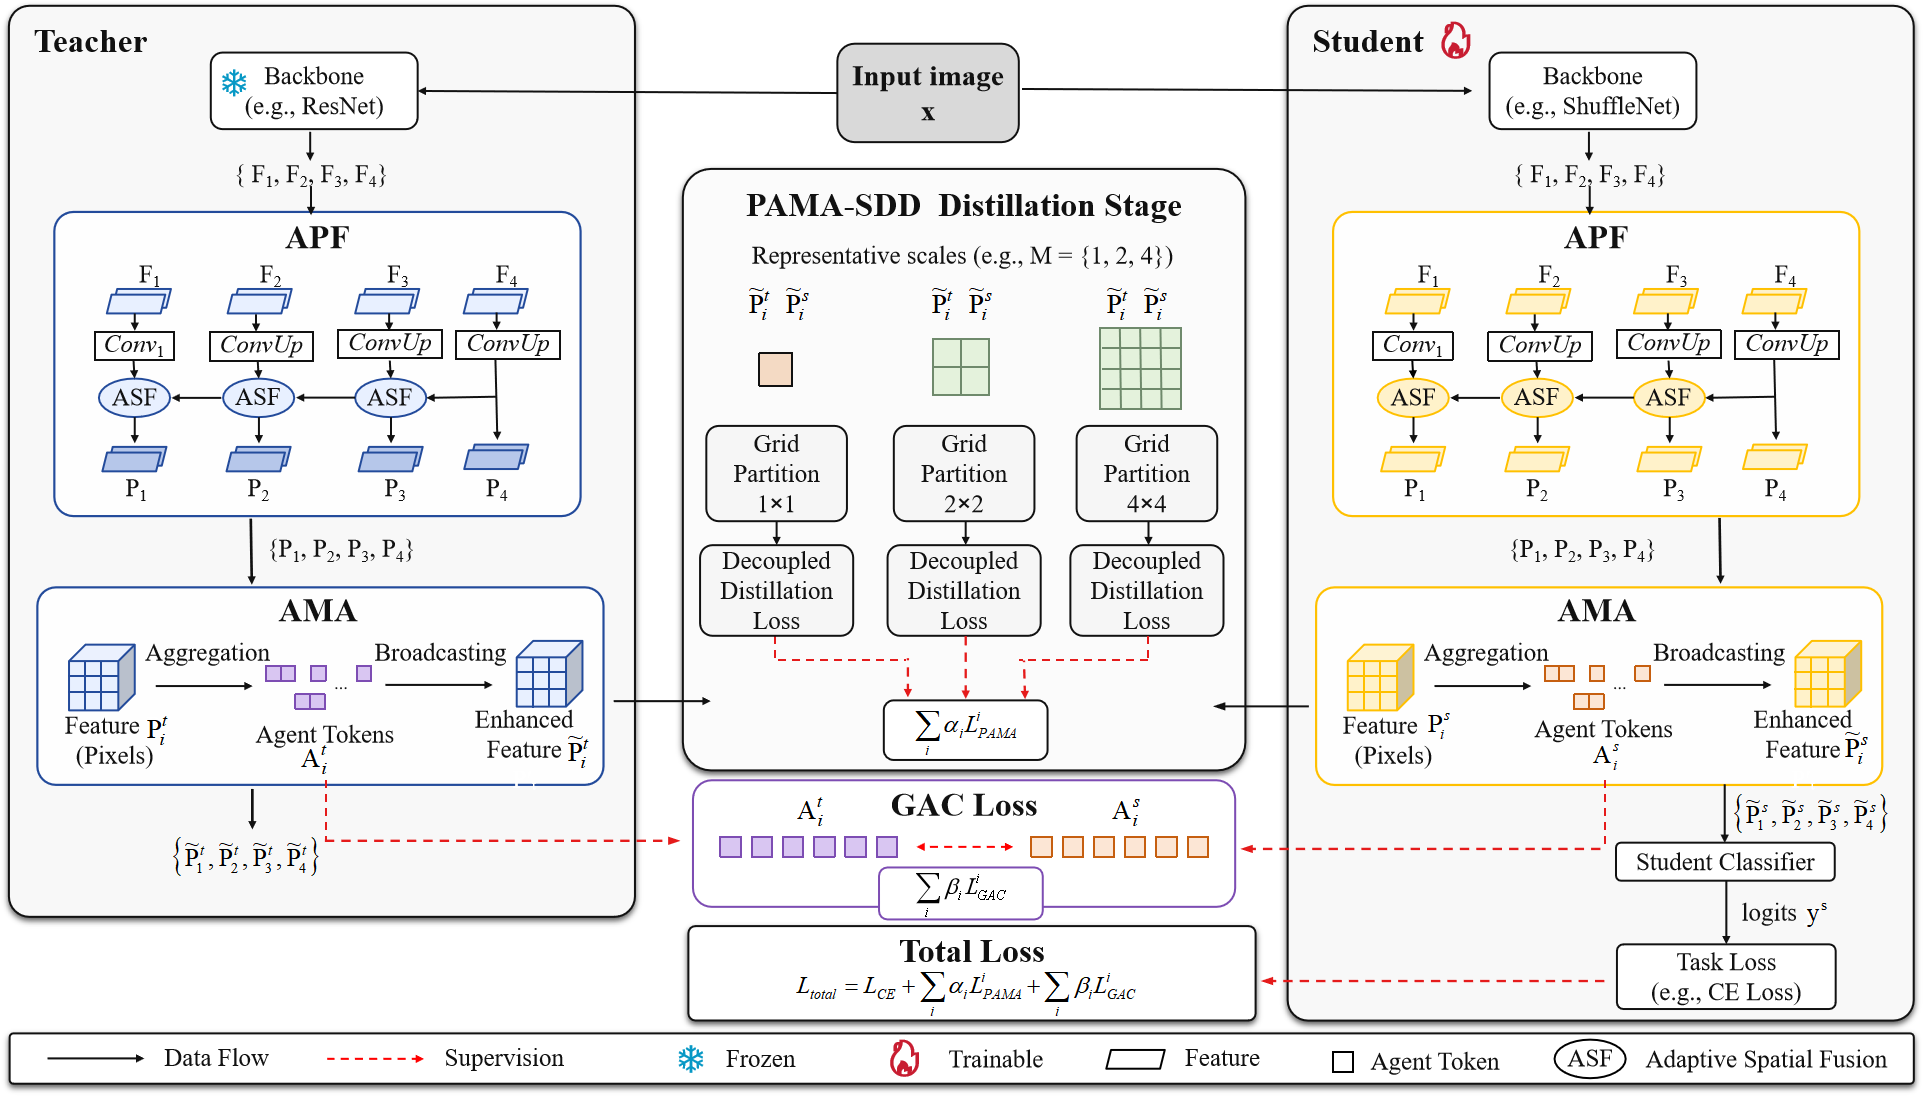
\includegraphics[width=\textwidth]{figs/overview1.png}
    \caption{
    Overall framework of PAMA-SDD++. The frozen teacher provides stable
    global logits, local logits, and non-parametric agent relations. The
    trainable student first builds a calibrated pyramid with PSPC, then uses
    CSAM to mediate global context through cross-scale agents. The training
    objective combines global KD, reliability-aware local distillation,
    local-global coherence, and relation-graph GAC. During inference, only
    the trained student network is retained.
    }
    \label{fig:overview}
\end{figure*}

Fig.~\ref{fig:overview} gives the training pipeline. PAMA-SDD++ separates the
roles of teacher and student deliberately. The teacher is a fixed reference:
it provides the image-level distribution, local logits induced by its own
classifier, and a non-parametric agent relation graph. No trainable
teacher-side pyramid or attention module is added, so the target does not move
while the student is being optimized. The student contains all mediation
modules, and these modules are removed after training.

The student path has two stages before the losses are evaluated. PSPC first
calibrates the hierarchy of student features, allowing local logits to be
computed from a pyramid in which fine spatial detail has access to deeper
semantic context. CSAM then summarizes the calibrated pyramid with compact
agents, lets the agents collect evidence from local regions, and broadcasts
the resulting global context back to the region tokens. The objective closes
the loop: reliability-aware local distillation selects trustworthy regional
teacher signals, LGC prevents local predictions from drifting away from the
teacher's global belief, and GAC transfers the relation structure among
agents. Thus, the method keeps the main advantage of SDD--explicit local
evidence--while reducing the two sources of error introduced by grid
partitioning: unreliable regions and fragmented semantics.

\subsection{Problem Formulation and Stable Teacher Targets}

Let $\mathcal{D}=\{(x_n,y_n)\}_{n=1}^{N_d}$ be a training set with $C$
classes. Knowledge distillation trains a compact student network
$\mathcal{S}$ under the supervision of a pretrained teacher network
$\mathcal{T}$. For an input image $x$, the teacher and student output
classification logits and four-level backbone features, as illustrated in
Fig.~\ref{fig:overview}:
\begin{equation}
\begin{split}
    (z^{t},\{F_i^{t}\}_{i=1}^{4})&=\mathcal{T}(x),\\
    (z^{s},\{F_i^{s}\}_{i=1}^{4})&=\mathcal{S}(x),
\end{split}
\label{eq:problem_formulation}
\end{equation}
where the superscripts $t$ and $s$ denote teacher and student branches,
respectively, $z^b\in\mathbb{R}^{C}$ is the classification logit, and
$F_i^b\in\mathbb{R}^{C_i^b\times H_i\times W_i}$ is the $i$-th backbone
feature of branch $b\in\{t,s\}$. The teacher parameters are fixed throughout
training, and all teacher-side representations are detached from gradient
updates.

The stable teacher path provides three targets. The global logit $z^t$
encodes the teacher's image-level class distribution. The final teacher
feature $F_4^t$ is partitioned into multi-scale regions and mapped by the
teacher classifier to produce local logits. Non-parametric teacher agents are
obtained by adaptive average pooling:
\begin{equation}
    A^{t}=\operatorname{Flatten}\left(
    \operatorname{AAP}_{h_a\times w_a}(F_4^t)\right)
    \in\mathbb{R}^{M\times C_4^t},
\label{eq:teacher_agents}
\end{equation}
where $M=h_aw_a$ is the number of agents. Because these agents are pooled
directly from the frozen teacher feature, their relation graph is a stable
semantic target even when teacher and student channel dimensions differ.

Conventional logit distillation transfers only image-level prediction
knowledge from $z^t$ to $z^s$. SDD makes the supervision spatially explicit,
but fixed partitions may be unreliable and independently optimized local
predictions may be weakly coupled with the teacher's global semantics.
PAMA-SDD++ keeps the classification-oriented local-logit interface of SDD and
adds the mediation machinery needed to make the local targets reliable and
globally coherent.

\subsection{Progressive Semantic Pyramid Calibration}

\begin{figure}[pos=t]
    \centering
    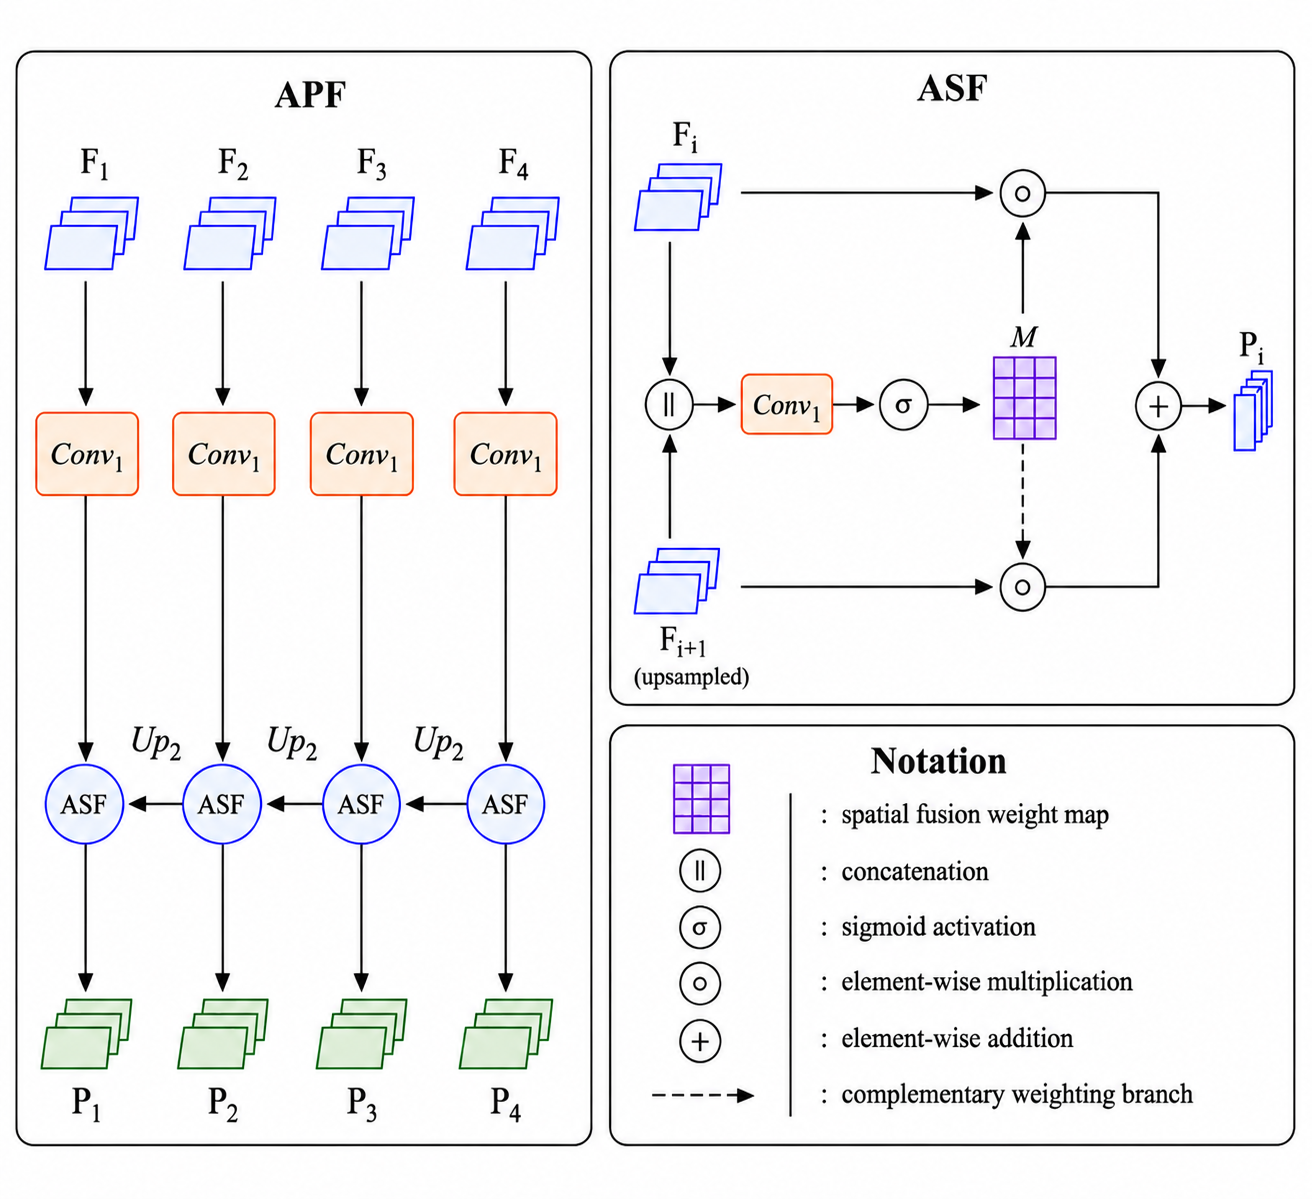
\includegraphics[width=0.98\columnwidth]{figs/APF.png}
    \caption{
    Schematic structure of PSPC. Each student backbone feature is projected
    into a shared channel space. Deep semantic context is progressively
    propagated to finer levels by channel-spatial adaptive fusion, whose gate
    predicts a $C'\times H\times W$ reliability map and uses a residual scale
    for stable optimization.
    }
    \label{fig:apf_module}
\end{figure}

Local logits inherit the quality of the feature maps from which they are
generated. Shallow features preserve spatial detail but can lack class-level
semantics; deep features are semantic but spatially coarse. PSPC reduces this
mismatch before any grid partition is applied. Unlike a generic feature neck,
it is used only to calibrate the student during distillation, and its outputs
are consumed by both local-logit construction and CSAM.

The student feature at each level is first projected into a shared channel
space:
\begin{equation}
    \bar{F}_i^{s}=\psi_i^{s}(F_i^{s}),
    \qquad i=1,2,3,4,
\label{eq:apf_projection}
\end{equation}
where $\psi_i^s(\cdot)$ denotes a $1\times1$ convolutional projection. The
deepest projected feature initializes the top-down fusion path:
\begin{equation}
    P_4^{s}=\bar{F}_4^{s}.
\label{eq:apf_init}
\end{equation}
For $i=3,2,1$, the deeper calibrated feature is upsampled to the spatial
resolution of the current level:
\begin{equation}
    U_{i+1}^{s}=\operatorname{Up}(P_{i+1}^{s};H_i,W_i),
\label{eq:apf_upsample}
\end{equation}
where $\operatorname{Up}(\cdot)$ denotes bilinear upsampling. A channel-spatial
gate then estimates how much current-level detail and deeper semantic context
should be retained at each location and channel:
\begin{equation}
    M_i^{s}=\sigma\left(\omega_i^{s}
    \left([\bar{F}_i^{s},U_{i+1}^{s}]\right)\right),
    \quad
    M_i^s\in[0,1]^{C'\times H_i\times W_i},
\label{eq:asf_mask}
\end{equation}
where $[\cdot,\cdot]$ denotes channel-wise concatenation,
$\omega_i^s(\cdot)$ is a lightweight convolutional transformation, and
$\sigma(\cdot)$ is the sigmoid activation. The fused feature is injected
through a learnable residual scale:
\begin{equation}
    \hat{P}_i^{s}=M_i^{s}\odot \bar{F}_i^{s}
    +(1-M_i^{s})\odot U_{i+1}^{s},
    \qquad
    P_i^s=\bar{F}_i^s+\gamma_i(\hat{P}_i^s-\bar{F}_i^s),
\label{eq:asf_fusion}
\end{equation}
where $\odot$ denotes element-wise multiplication and $\gamma_i$ is a
learnable residual scale. The output of PSPC is the calibrated student
pyramid $\mathcal{P}^s=\{P_1^s,P_2^s,P_3^s,P_4^s\}$.

\subsection{Cross-Scale Agent Mediation}

\begin{figure*}[pos=t]
    \centering
    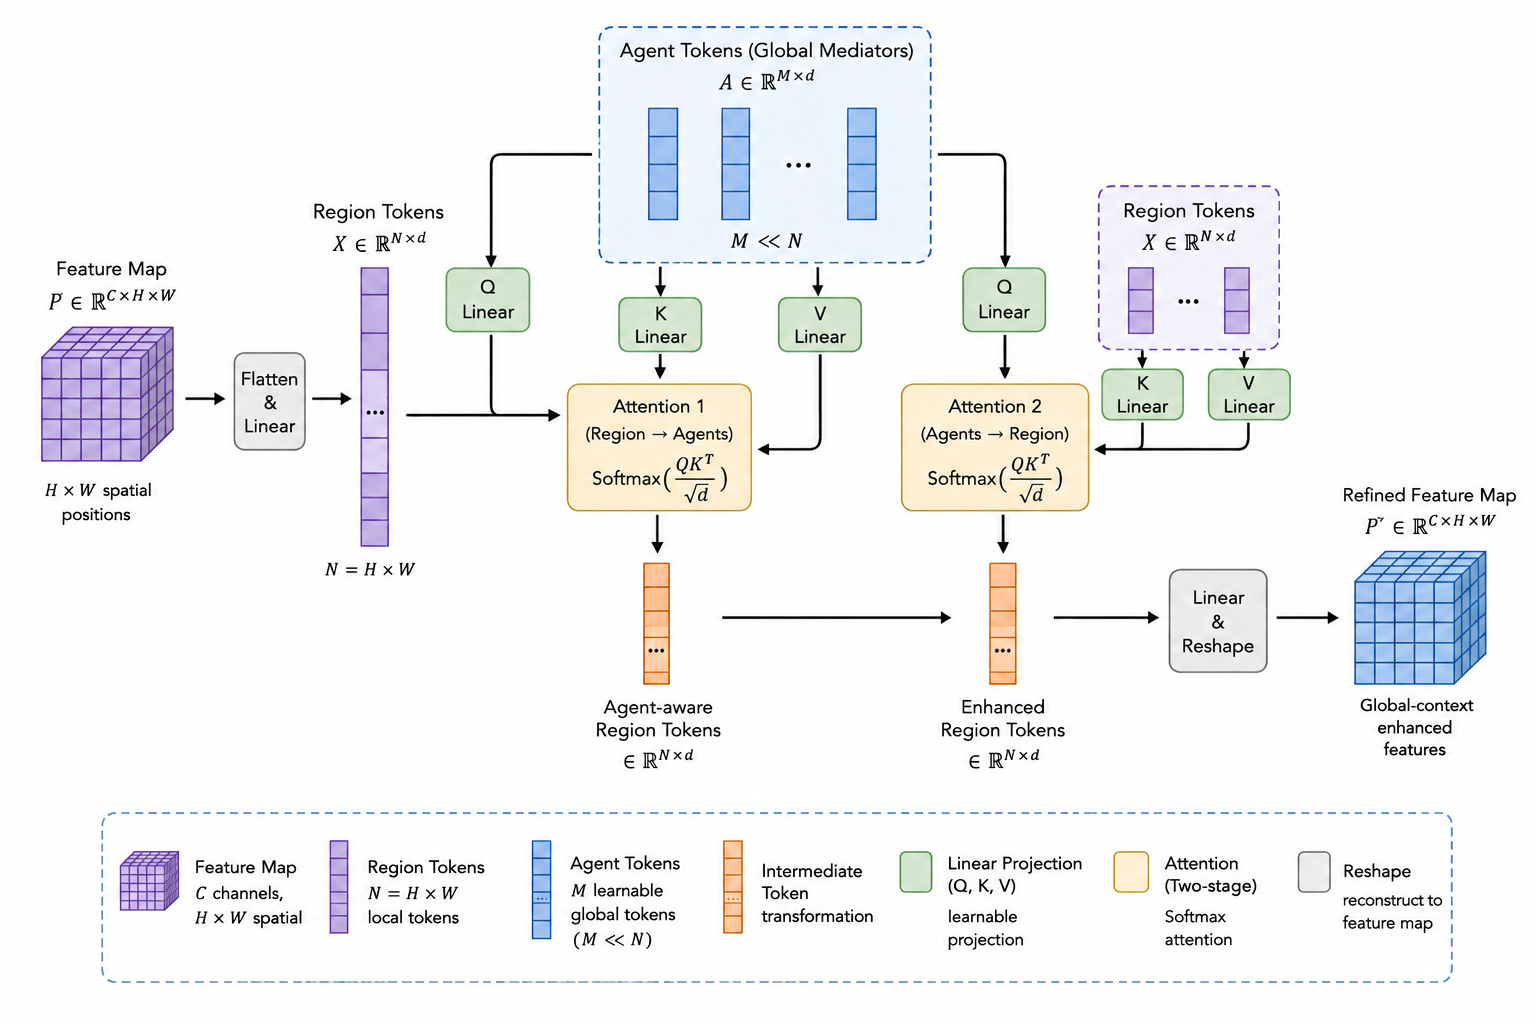
\includegraphics[width=0.98\textwidth]{figs/AMA1.png}
    \caption{
    Schematic structure of CSAM. The finest PSPC feature is flattened into
    region tokens, while ordered agent tokens are initialized from all
    calibrated pyramid levels with learnable scale weights. Agents first
    aggregate region information and then broadcast global context back to
    local tokens. A depth-wise local branch preserves convolutional local
    inductive bias.
    }
    \label{fig:ama_module}
\end{figure*}

PSPC prepares the feature pyramid, but the local logits are still defined on
grid regions. If those regions remain isolated, the student can improve local
discrimination while losing global consistency. Dense region-to-region
self-attention would address the interaction problem, but it is expensive for
high-resolution maps. CSAM uses a compact alternative: a small set of ordered
agents mediates the communication between local regions. The agents are
initialized from all calibrated pyramid levels, so they summarize fine spatial
evidence and coarse semantic context before returning global information to
the local tokens.

Let the finest calibrated feature $P_1^s\in\mathbb{R}^{C'\times H_1\times W_1}$
be the base feature for local enhancement. CSAM first obtains region tokens:
\begin{equation}
    X^{s}=\operatorname{Flatten}(P_1^s)
    \in\mathbb{R}^{N\times C'},
    \qquad N=H_1W_1.
\label{eq:ama_region_tokens}
\end{equation}
For each pyramid level, ordered agent evidence is obtained by adaptive average
pooling. The pooled evidence is aggregated with learnable softmax-normalized
scale weights:
\begin{equation}
\begin{split}
    B_l^s &= \operatorname{Flatten}
    \left(\operatorname{AAP}_{h_a\times w_a}(P_l^s)\right),\\
    \rho_l &= \frac{\exp(r_l)}{\sum_{q=1}^{4}\exp(r_q)},\\
    A_0^s &= \phi_a\left(\sum_{l=1}^{4}\rho_l B_l^s\right)+E,
    \qquad M=h_aw_a,
\end{split}
\label{eq:ama_agent_init}
\end{equation}
where $r_l$ are learnable scale logits, $\phi_a(\cdot)$ is a linear
projection, $E\in\mathbb{R}^{M\times C'}$ is a learnable semantic prototype,
and $M\ll N$.

CSAM contains two attention stages. In the aggregation stage, agent tokens
serve as queries, while region tokens provide keys and values:
\begin{equation}
    A^{s}=\operatorname{LN}\left(A_0^{s}+
    \operatorname{Attn}(A_0^{s},X^{s},X^{s})\right).
\label{eq:ama_aggregation}
\end{equation}
In the broadcasting stage, region tokens query the updated agents and receive
agent-mediated global context:
\begin{equation}
    \hat{X}^{s}=X^{s}+
    \gamma\odot W_o
    \operatorname{Attn}(\operatorname{LN}(X^{s}),A^{s},A^{s}),
\label{eq:ama_broadcast}
\end{equation}
where $\gamma$ is a LayerScale parameter. For a single attention head, the
attention operation is
\begin{equation}
    \operatorname{Attn}(Q,K,V)=
    \operatorname{Softmax}\left(\frac{QW_Q(KW_K)^\top}{\sqrt{d_h}}\right)VW_V,
\label{eq:attention}
\end{equation}
where $W_Q$, $W_K$, and $W_V$ are learnable projection matrices and $d_h$ is
the head dimension. The enhanced tokens are reshaped into a refined feature
map and combined with a depth-wise local positional branch:
\begin{equation}
    \tilde{P}_1^{s}=\operatorname{Reshape}(\hat{X}^{s})
    +\operatorname{DWConv}(P_1^s).
\label{eq:ama_output}
\end{equation}
CSAM outputs the enhanced student feature $\tilde{P}_1^s$ for local logits
and agent tokens $A^s$ for relation-graph distillation.

\subsection{Training Objective and Optimization}

The training objective contains five terms: standard classification, global
logit distillation, reliability-aware local distillation, local-global
coherence, and relation-graph agent consistency. The standard classification
loss is
\begin{equation}
    \mathcal{L}_{\operatorname{CE}}=\operatorname{CE}(z^s,y),
\label{eq:loss_ce}
\end{equation}
where $y$ is the ground-truth label. The global distillation loss is denoted
as $\mathcal{L}_{\operatorname{global}}=
\mathcal{D}_{\operatorname{base}}(z^s,z^t,y;\tau)$, where
$\mathcal{D}_{\operatorname{base}}$ can be instantiated as KD, DKD, or NKD.

Let $\mathcal{M}=\{m_1,m_2,\ldots,m_K\}$ denote the representative grid scale
set, e.g., $\{1,2,4\}$ in Fig.~\ref{fig:overview}. Each grid scale is paired
with a student pyramid level through a scale-aware mapping $\pi(m_i)$. The
finest feature uses $\tilde{P}_1^s$, while other scales use the PSPC
calibrated pyramid. Grid partition then produces local regions:
\begin{equation}
    \mathcal{G}_{i}^{s}=\operatorname{Grid}_{m_i\times m_i}
    (Q_{\pi(m_i)}^{s})=
    \{g_{i,j}^{s}\}_{j=1}^{m_i^2},
\label{eq:grid_partition}
\end{equation}
where $Q^s=\{\tilde{P}_1^s,P_2^s,P_3^s,P_4^s\}$. Each student region is
converted into a local classification logit by the student classifier:
\begin{equation}
    \ell_{i,j}^{s}=h^{s}(g_{i,j}^{s}),
    \qquad j=1,\ldots,m_i^2,
\label{eq:local_logits}
\end{equation}
where $h^s(\cdot)$ is the student classifier. Teacher local logits are
obtained from the frozen final teacher feature:
\begin{equation}
    \ell_{i,j}^{t}=h^{t}\left(
    \operatorname{Grid}_{m_i\times m_i}(F_4^t)_j\right),
    \qquad j=1,\ldots,m_i^2.
\label{eq:teacher_local_logits}
\end{equation}
All local logits are concatenated into tensors
$L^s,L^t\in\mathbb{R}^{B\times C\times N}$, where $N=\sum_i m_i^2$.

RA-PAMA estimates the reliability of each teacher local target from its local
confidence:
\begin{equation}
\begin{aligned}
    p_n^t&=\operatorname{Softmax}(\ell_n^t/\tau),\\
    r_n&=\operatorname{Clamp}\left(
    \frac{\max_c p_{n,c}^t-1/C}{1-1/C},0,1\right),
\end{aligned}
\label{eq:region_reliability}
\end{equation}
where $n$ indexes all local regions. The final weight retains a floor value so
that difficult regions are not completely discarded:
\begin{equation}
    w_n=\lambda_{\min}+(1-\lambda_{\min})r_n^{\eta}.
\label{eq:region_weight}
\end{equation}
The reliability-aware PAMA loss is
\begin{equation}
    \mathcal{L}_{\operatorname{PAMA}}
    =
    \frac{\sum_{n=1}^{N}w_n
    \mathcal{D}_{\operatorname{base}}(\ell_n^s,\ell_n^t,y;\tau)}
    {\sum_{n=1}^{N}w_n}.
\label{eq:loss_pama}
\end{equation}
This weighting keeps hard but informative regions in the loss through the
floor value, while reducing the influence of partitions whose teacher
prediction is close to uniform or dominated by background.

LGC further constrains local student predictions by the teacher global
distribution:
\begin{equation}
\begin{aligned}
    \mathcal{L}_{\operatorname{LGC}}
    &=\frac{\sum_{n=1}^{N}w_n d_n^{\operatorname{lgc}}}
    {\sum_{n=1}^{N}w_n},\\
    d_n^{\operatorname{lgc}}
    &=\tau^2\operatorname{KL}\left(
    \operatorname{Softmax}(z^t/\tau)
    \,\|\,\operatorname{Softmax}(\ell_n^s/\tau)\right).
\end{aligned}
\label{eq:loss_lgc}
\end{equation}
This term discourages local predictions from drifting away from the teacher's
image-level semantic distribution.

GAC provides a complementary constraint in the agent-relation space. Let
$A^s\in\mathbb{R}^{M\times C_4^s}$ and
$A^t\in\mathbb{R}^{M\times C_4^t}$ denote the student and teacher agents.
Because teacher and student channels can be different, PAMA-SDD++ aligns
their relation graphs rather than raw token features:
\begin{equation}
\begin{aligned}
    R^s&=\operatorname{Norm}(A^s)\operatorname{Norm}(A^s)^\top,\\
    R^t&=\operatorname{Norm}(A^t)\operatorname{Norm}(A^t)^\top .
\end{aligned}
\label{eq:gac_relation}
\end{equation}
The relation-graph GAC loss is
\begin{equation}
\begin{aligned}
    \mathcal{L}_{\operatorname{GAC}}
    &=
    \tau_g^2
    \operatorname{KL}\left(P_R^t\,\|\,P_R^s\right)
    +\|R^s-\operatorname{sg}(R^t)\|_F^2,\\
    P_R^b&=\operatorname{Softmax}(R^b/\tau_g),\quad b\in\{s,t\}.
\end{aligned}
\label{eq:loss_gac}
\end{equation}
where $\operatorname{sg}(\cdot)$ denotes the stop-gradient operation. GAC
transfers how teacher agents relate to one another, which is more
architecture-agnostic than direct feature matching.

The distillation losses are warmed up during early training:
\begin{equation}
    \mu(e)=\min\left(\frac{e+1}{E_w},1\right),
\label{eq:warmup}
\end{equation}
where $e$ is the epoch index and $E_w$ is the warmup length. The final
objective is
\begin{equation}
\begin{aligned}
    \mathcal{L}_{\operatorname{total}}
    &=
    \lambda_{\operatorname{ce}}\mathcal{L}_{\operatorname{CE}}\\
    &\quad+\mu(e)\left(
    \lambda_{\operatorname{g}}\mathcal{L}_{\operatorname{global}}
    +\lambda_{\operatorname{p}}\mathcal{L}_{\operatorname{PAMA}}
    +\lambda_{\operatorname{c}}\mathcal{L}_{\operatorname{LGC}}
    +\lambda_{\operatorname{a}}\mathcal{L}_{\operatorname{GAC}}
    \right).
\end{aligned}
\label{eq:loss_total}
\end{equation}
where the $\lambda$ terms balance the corresponding losses. During
optimization, gradients update the student and the training-only PSPC/CSAM
modules, while all teacher targets remain detached.

\subsection{Inference Procedure}

PAMA-SDD++ uses PSPC, CSAM, RA-PAMA, LGC, and GAC only to improve student
training. After training, the teacher branch, auxiliary distillation modules,
local-logit computations, and loss terms are removed. As shown in
Fig.~\ref{fig:overview}, prediction is performed by the original student
network alone. Therefore, the deployed model has the same inference cost as
the student baseline.

\section{Experiments}
\label{sec:experiments}

\subsection{Experimental Setup}
\label{subsec:experimental_setup}

\subsubsection{Datasets and Evaluation Metrics}
We evaluate PAMA-SDD++ on CIFAR-100~\cite{krizhevsky2009learning},
ImageNet-1K~\cite{deng2009imagenet}, and
CUB-200-2011~\cite{wah2011cub}. The three benchmarks stress different parts
of the method. CIFAR-100 covers a broad set of teacher--student architecture
pairs under a standard small-scale protocol. ImageNet-1K tests whether the
local--global design remains useful at large scale. CUB-200-2011 is a
fine-grained benchmark in which part-level evidence and object-level semantic
consistency are both decisive.

CIFAR-100 contains 50,000 training images and 10,000 test images from 100
classes. ImageNet-1K follows the ILSVRC-2012 classification setting and uses
the validation set for evaluation. CUB-200-2011 contains 200 bird categories.
We report top-1 accuracy on CIFAR-100 and CUB-200-2011, and both top-1 and
top-5 accuracy on ImageNet-1K. All values are percentages.

\subsubsection{Compared Methods}
We compare PAMA-SDD++ with representative response-based, feature-based,
relation-based, contrastive, and scale-decoupled distillation methods:
KD~\cite{hinton2015distilling}, FitNet~\cite{romero2015fitnets},
RKD~\cite{park2019relational}, SP~\cite{tung2019similarity},
PKT~\cite{passalis2018learning}, CRD~\cite{tian2020contrastive},
WCoRD~\cite{chen2021wasserstein}, SemCKD~\cite{chen2021semckd},
ReviewKD~\cite{chen2021distilling}, MGD~\cite{yang2022masked},
DKD~\cite{zhao2022decoupled}, NKD~\cite{yang2023knowledge}, and
SDD~\cite{wei2024scaled}. To contextualize the results with recent
high-performing baselines, we also include GDKD~\cite{zheng2025rethinking}
and RLD~\cite{sun2025knowledge} when their reported teacher--student settings
overlap with ours. Entries unavailable in the original reports are denoted by
``--''. Because PAMA-SDD++ enhances SDD rather than replacing the base logit
objective, we instantiate it with KD, DKD, and NKD, obtaining PAMA++-KD,
PAMA++-DKD, and PAMA++-NKD. These variants are compared with SD-KD, SD-DKD,
and SD-NKD under the same base objective.

\subsubsection{Implementation Details}
The teacher backbone is fixed throughout distillation. It provides global
logits, local logits from its final feature and classifier, and pooled
non-parametric agent relations. PSPC, CSAM, local-logit construction, RA-PAMA,
LGC, and GAC are training-only components. At test time they are discarded,
leaving the original student classifier and therefore the same deployment cost
as the student baseline.

Unless otherwise stated, the local scale set is $\{1,2,4\}$, the number of
agents is 16, and CSAM uses 4 attention heads. We use temperature 4.0, a
30-epoch warmup for distillation losses, reliability floor 0.2, reliability
power 1.0, PSPC residual-scale initialization 0.5, and CSAM LayerScale
initialization $10^{-4}$. The loss coefficients follow the corresponding
released configuration; ablations explicitly state the varied coefficient.
Mixed-precision training is enabled when supported, and gradient clipping with
maximum norm 5.0 is used for numerical stability. CIFAR-100 models are trained
for 240 epochs with SGD, momentum 0.9, weight decay $5\times10^{-4}$, batch
size 64, and learning-rate decay at epochs 150, 180, and 210. ImageNet-1K
models are trained for 100 epochs with batch size 512 and learning-rate decay
at epochs 30, 60, and 90. CUB-200-2011 models are trained for 240 epochs with
the same staged learning-rate schedule as CIFAR-100.

\subsection{Quantitative Comparison Results}

\subsubsection{Results on CIFAR-100}

\begin{table*}[pos=t]
\centering
\small
\caption{Top-1 accuracy (\%) on CIFAR-100 for teacher--student pairs with different feature-level configurations. The best student result in each column is highlighted in bold.}
\label{tab:cifar_diff_level}
\setlength{\tabcolsep}{4pt}
\resizebox{\textwidth}{!}{
\begin{tabular}{lcccc}
\toprule
\textbf{Method} 
& \textbf{ResNet32x4 $\rightarrow$ MobileNetV2} 
& \textbf{WRN-40-2 $\rightarrow$ VGG8} 
& \textbf{WRN-40-2 $\rightarrow$ MobileNetV2} 
& \textbf{ResNet50 $\rightarrow$ ShuffleNetV1} \\
\midrule
Teacher  & 79.42 & 75.61 & 75.61 & 79.34 \\
Student  & 64.60 & 70.36 & 64.60 & 70.50 \\
\midrule
FitNet~\cite{romero2015fitnets}   & 65.61 & 70.98 & 65.12 & 72.03 \\
SP~\cite{tung2019similarity}       & 67.52 & 73.18 & 66.34 & 71.28 \\
CRD~\cite{tian2020contrastive}      & 69.13 & 73.88 & 68.89 & 75.70 \\
SemCKD~\cite{chen2021semckd}   & 68.99 & 73.67 & 68.34 & 75.56 \\
MGD~\cite{yang2022masked}      & 68.13 & 73.33 & 68.55 & 74.99 \\
RLD~\cite{sun2025knowledge}    & -- & -- & 69.75 & -- \\
\midrule
KD~\cite{hinton2015distilling}       & 67.72 & 73.97 & 68.87 & 75.82 \\
SD-KD~\cite{wei2024scaled}    & 68.84 & 74.44 & 69.81 & 76.87 \\
PAMA++-KD  & 69.75 {\scriptsize (+0.91)} 
         & \textbf{75.22} {\scriptsize (+0.78)} 
         & 70.45 {\scriptsize (+0.64)} 
         & 78.29 {\scriptsize (+1.42)} \\
\midrule
DKD~\cite{zhao2022decoupled}      & 68.98 & 74.13 & 69.33 & 77.01 \\
SD-DKD~\cite{wei2024scaled}   & 70.08 & 74.58 & 70.13 & 78.11 \\
PAMA++-DKD & \textbf{71.10} {\scriptsize (+1.02)} 
         & 75.00 {\scriptsize (+0.42)} 
         & 71.17 {\scriptsize (+1.04)} 
         & \textbf{79.70} {\scriptsize (+1.59)} \\
\midrule
NKD~\cite{yang2023knowledge}      & 68.81 & 73.80 & 68.85 & 76.22 \\
SD-NKD~\cite{wei2024scaled}   & 69.59 & 74.34 & 70.04 & 76.95 \\
PAMA++-NKD & 70.42 {\scriptsize (+0.83)} 
         & 74.75 {\scriptsize (+0.41)} 
         & \textbf{71.49} {\scriptsize (+1.45)} 
         & 78.74 {\scriptsize (+1.79)} \\
\bottomrule
\end{tabular}
}
\vspace{2pt}
\begin{minipage}{0.98\textwidth}
\footnotesize
\textit{Note:} The values in parentheses denote the absolute improvement over the corresponding scale-decoupled baseline, i.e., SD-KD, SD-DKD, or SD-NKD. Recent-method results are taken from their original papers; ``--'' denotes unavailable reported settings.
\end{minipage}
\end{table*}

CIFAR-100 evaluates the general applicability of PAMA-SDD++ across diverse
teacher--student architectures. We report two groups of results. The first
group contains pairs with different feature-level configurations, where
feature-space mismatch is more pronounced. The second group contains pairs
with more aligned feature hierarchies. This organization allows us to
examine whether reliability-aware pyramid-agent mediation is useful under
both heterogeneous and relatively aligned distillation settings.



As shown in Table~\ref{tab:cifar_diff_level}, all PAMA variants improve
their corresponding scale-decoupled baselines in the different-level
settings. PAMA++-KD improves SD-KD by 0.64--1.42 percentage points,
PAMA++-DKD improves SD-DKD by 0.42--1.59 points, and PAMA++-NKD improves
SD-NKD by 0.41--1.79 points. For the overlapping
WRN-40-2$\rightarrow$MobileNetV2 setting, PAMA++-NKD is 1.74 points higher
than RLD. The gains across KD, DKD, and NKD indicate
that PAMA-SDD++ is not tied to a single base distillation objective. Instead,
PSPC, CSAM, RA-PAMA, LGC, and relation-graph GAC provide complementary
feature calibration, local reliability modeling, and semantic alignment for
scale-decoupled local logit transfer.

\begin{table*}[pos=t]
\centering
\small
\caption{Top-1 accuracy (\%) on CIFAR-100 for teacher--student pairs with the same feature-level configurations. The best student result in each column is highlighted in bold.}
\label{tab:cifar_same_level}
\setlength{\tabcolsep}{3pt}
\resizebox{\textwidth}{!}{
\begin{tabular}{lcccccc}
\toprule
\textbf{Method} 
& \textbf{RN32x4 $\rightarrow$ ShuNetV1} 
& \textbf{WRN-40-2 $\rightarrow$ ShuNetV1} 
& \textbf{RN50 $\rightarrow$ MobNetV2} 
& \textbf{VGG13 $\rightarrow$ MobNetV2} 
& \textbf{RN32x4 $\rightarrow$ ShuNetV2} 
& \textbf{RN50 $\rightarrow$ VGG8} \\
\midrule
Teacher  & 79.42 & 75.61 & 75.61 & 79.34 & 79.42 & 75.61 \\
Student  & 70.50 & 70.50 & 64.60 & 64.60 & 71.82 & 70.36 \\
\midrule
FitNet~\cite{romero2015fitnets}   & 73.54 & 73.73 & 63.16 & 63.16 & 73.54 & 70.69 \\
RKD~\cite{park2019relational}      & 72.28 & 72.21 & 64.43 & 64.43 & 73.21 & 71.50 \\
SP~\cite{tung2019similarity}       & 73.48 & 74.52 & 68.08 & 68.08 & 74.56 & 73.34 \\
PKT~\cite{passalis2018learning}      & 74.10 & 72.21 & 66.52 & 66.52 & 74.69 & 73.01 \\
CRD~\cite{tian2020contrastive}      & 75.11 & 76.05 & 69.11 & 69.11 & 75.65 & 74.30 \\
WCoRD~\cite{chen2021wasserstein}    & 75.77 & 76.32 & 70.45 & 69.47 & 75.96 & 74.86 \\
SemCKD~\cite{chen2021semckd}   & 76.31 & 76.06 & 68.69 & 69.98 & 77.02 & 74.18 \\
ReviewKD~\cite{chen2021distilling} & 77.45 & 77.14 & 69.89 & 70.37 & 77.78 & 75.34 \\
MGD~\cite{yang2022masked}      & 76.22 & 75.89 & 68.54 & 69.44 & 76.65 & 73.89 \\
GDKD~\cite{zheng2025rethinking} & 78.21 & \textbf{78.05} & 70.55 & 70.35 & \textbf{79.27} & -- \\
RLD~\cite{sun2025knowledge}    & --    & --    & 70.76 & 69.97 & 77.56 & -- \\
\midrule
KD~\cite{hinton2015distilling}       & 74.07 & 74.83 & 67.35 & 67.37 & 74.45 & 73.81 \\
SD-KD~\cite{wei2024scaled}    & 76.30 & 76.65 & 69.55 & 68.79 & 76.67 & 74.89 \\
PAMA++-KD  & 77.63 {\scriptsize (+1.33)} 
         & 77.36 {\scriptsize (+0.71)} 
         & 70.49 {\scriptsize (+0.94)} 
         & 69.70 {\scriptsize (+0.91)} 
         & 76.40 {\scriptsize ($-0.27$)} 
         & 75.29 {\scriptsize (+0.40)} \\
\midrule
DKD~\cite{zhao2022decoupled}      & 76.45 & 76.70 & 70.35 & 69.71 & 77.07 & 75.34 \\
SD-DKD~\cite{wei2024scaled}   & 77.30 & 77.21 & 71.36 & 70.25 & 78.05 & 75.86 \\
PAMA++-DKD & \textbf{79.18} {\scriptsize (+1.88)} 
         & 77.43 {\scriptsize (+0.22)} 
         & \textbf{71.80} {\scriptsize (+0.44)} 
         & \textbf{71.22} {\scriptsize (+0.97)} 
         & 78.50 {\scriptsize (+0.45)} 
         & \textbf{76.45} {\scriptsize (+0.59)} \\
\midrule
NKD~\cite{yang2023knowledge}      & 75.31 & 75.96 & 69.39 & 68.72 & 76.26 & 74.01 \\
SD-NKD~\cite{wei2024scaled}   & 76.34 & 76.81 & 70.25 & 69.50 & 77.07 & 74.62 \\
PAMA++-NKD & 76.86 {\scriptsize (+0.52)} 
         & 77.61 {\scriptsize (+0.80)} 
         & 71.48 {\scriptsize (+0.23)} 
         & 70.58 {\scriptsize (+1.08)} 
         & 77.39 {\scriptsize (+0.32)} 
         & 75.03 {\scriptsize (+0.41)} \\
\bottomrule
\end{tabular}
}
\vspace{2pt}
\begin{minipage}{0.98\textwidth}
\footnotesize
\textit{Note:} RN, WRN, ShuNet, and MobNet denote ResNet, WideResNet, ShuffleNet, and MobileNet, respectively. The values in parentheses denote the absolute improvement over the corresponding scale-decoupled baseline. Recent-method results are taken from their original papers; ``--'' denotes unavailable reported settings.
\end{minipage}
\end{table*}

Table~\ref{tab:cifar_same_level} reports the same-level settings. PAMA-SDD++
again improves most SD baselines. With recent methods included, PAMA++-DKD
obtains the best student accuracy in four of the six settings and improves
SD-DKD by 0.22--1.88 percentage points. GDKD is stronger in two
ShuffleNet-related settings, but PAMA++-DKD still surpasses both GDKD and RLD
when the student is MobileNetV2 under the ResNet50 and VGG13 teachers. These
results suggest that the proposed
modules are not only useful for compensating severe architectural mismatch;
they also improve distillation when teacher and student feature hierarchies
are relatively aligned. Overall, the CIFAR-100 results support the central
motivation of PAMA-SDD++: local scale-decoupled supervision benefits from
reliable local targets, semantic feature calibration, and agent-level global
consistency.

\subsubsection{Results on ImageNet-1K}
\label{subsec:imagenet_results}

Table~\ref{tab:imagenet_results} reports the ImageNet-1K results under a
homogeneous pair, ResNet34$\rightarrow$ResNet18, and a heterogeneous pair,
ResNet50$\rightarrow$MobileNetV2. PAMA-SDD++ consistently improves the
corresponding SD variants in both top-1 and top-5 accuracy. For example,
PAMA++-DKD improves SD-DKD by 0.33 and 0.53 percentage points under
ResNet34$\rightarrow$ResNet18, and by 0.52 and 0.74 points under
ResNet50$\rightarrow$MobileNetV2. These results indicate that the proposed
local--global distillation design remains effective beyond small-scale
benchmarks.

\begin{table*}[pos=t]
\centering
\small
\setlength{\tabcolsep}{4pt}
\renewcommand{\arraystretch}{1.05}

\caption{Top-1 and top-5 accuracy (\%) on ImageNet-1K. Values in parentheses denote improvements over the corresponding SD baseline.}
\label{tab:imagenet_results}

\begin{tabular}{lcccc}
\toprule
\multirow{2}{*}{\textbf{Method}} & \multicolumn{2}{c}{\textbf{ResNet34 $\rightarrow$ ResNet18}} & \multicolumn{2}{c}{\textbf{ResNet50 $\rightarrow$ MobileNetV2}} \\
\cmidrule(lr){2-3}\cmidrule(lr){4-5}
 & \textbf{Top-1} & \textbf{Top-5} & \textbf{Top-1} & \textbf{Top-5} \\
\midrule
Teacher & 73.31 & 91.42 & 76.16 & 92.86 \\
Student & 69.75 & 89.07 & 68.87 & 88.76 \\
\midrule
GDKD~\cite{zheng2025rethinking} & 72.26 & 90.72 & 73.25 & 91.35 \\
RLD~\cite{sun2025knowledge} & 71.91 & 90.59 & 72.75 & 91.18 \\
\midrule
KD~\cite{hinton2015distilling} & 71.03 & 89.88 & 70.50 & 90.34 \\
SD-KD~\cite{wei2024scaled} & 71.44 & 90.05 & 72.24 & 90.71 \\
PAMA++-KD & 71.66 \gain{0.22} & 90.48 \gain{0.43} & 72.69 \gain{0.45} & 91.27 \gain{0.56} \\
\midrule
DKD~\cite{zhao2022decoupled} & 71.70 & 90.41 & 72.05 & 91.05 \\
SD-DKD~\cite{wei2024scaled} & 72.02 & 91.21 & 73.08 & 91.09 \\
PAMA++-DKD & 72.35 \gain{0.33} & \textbf{91.74} \gain{0.53} & \textbf{73.60} \gain{0.52} & \textbf{91.83} \gain{0.74} \\
\midrule
NKD~\cite{yang2023knowledge} & 71.96 & 91.10 & 73.08 & 91.09 \\
SD-NKD~\cite{wei2024scaled} & 72.33 & 91.31 & 73.12 & 91.11 \\
PAMA++-NKD & \textbf{72.57} \gain{0.24} & 91.42 \gain{0.11} & 73.44 \gain{0.32} & 91.73 \gain{0.62} \\
\bottomrule
\end{tabular}
\vspace{2pt}
\begin{minipage}{0.98\textwidth}
\footnotesize
\textit{Note:} Recent-method results are taken from their original papers. The values in parentheses denote improvements over the corresponding scale-decoupled baseline.
\end{minipage}
\end{table*}

Compared with recent methods, PAMA-SDD++ achieves competitive ImageNet-1K
performance. PAMA-SDD++ surpasses GDKD and RLD on all four ImageNet metrics.
In particular, PAMA++-DKD obtains the best top-5 accuracy under both evaluated
teacher--student pairs, while PAMA++-NKD and PAMA++-DKD achieve the best top-1
accuracy under ResNet34$\rightarrow$ResNet18 and
ResNet50$\rightarrow$MobileNetV2, respectively. This indicates that the proposed
local--global distillation design remains effective on large-scale
classification.

\subsubsection{Results on CUB-200-2011}
\label{subsec:cub_results}

CUB-200-2011 is used to evaluate fine-grained knowledge transfer. Different
bird categories often differ only in subtle regions such as the head, wing,
tail, or local texture. This benchmark therefore directly tests whether the
student can preserve local discriminative evidence while maintaining object-
level semantic consistency.

\begin{table*}[pos=t]
\centering
\caption{Top-1 accuracy (\%) on CUB-200-2011. Values in parentheses denote improvements over the corresponding SD baseline. The best result in each column is highlighted in bold.}
\label{tab:cub200_results}
\resizebox{\textwidth}{!}{
\begin{tabular}{lccccc}
\toprule
\textbf{Method} &
\textbf{ResNet32x4 $\rightarrow$ MobileNetV2} &
\textbf{ResNet32x4 $\rightarrow$ ShuffleNetV1} &
\textbf{VGG13 $\rightarrow$ MobileNetV2} &
\textbf{VGG13 $\rightarrow$ VGG8} &
\textbf{ResNet50 $\rightarrow$ ShuffleNetV1} \\
\midrule
Teacher & 66.17 & 66.17 & 70.19 & 70.19 & 60.01 \\
Student & 40.23 & 37.28 & 40.23 & 46.32 & 37.28 \\
\midrule
SP~\cite{tung2019similarity} & 48.49 & 61.83 & 44.28 & 54.78 & 55.31 \\
CRD~\cite{tian2020contrastive} & 57.45 & 62.28 & 56.45 & 66.10 & 57.45 \\
SemCKD~\cite{chen2021semckd} & 56.89 & 63.78 & 68.23 & 66.54 & 57.20 \\
ReviewKD~\cite{chen2021distilling} & -- & 64.12 & 58.66 & 67.10 & -- \\
MGD~\cite{yang2022masked} & -- & -- & -- & 66.89 & 57.12 \\
\midrule
KD~\cite{hinton2015distilling} & 56.09 & 61.68 & 53.98 & 64.18 & 57.21 \\
SD-KD~\cite{wei2024scaled} & 60.51 & 65.46 & 59.80 & 67.32 & 60.56 \\
PAMA++-KD & 63.62 \gain{3.11} & 66.14 \gain{0.68} & 61.98 \gain{2.18} & 68.57 \gain{1.25} & 61.13 \gain{0.57} \\
\midrule
DKD~\cite{zhao2022decoupled} & 59.94 & 64.51 & 58.45 & 67.20 & 59.21 \\
SD-DKD~\cite{wei2024scaled} & 62.97 & 65.58 & 64.86 & 68.67 & 60.66 \\
PAMA++-DKD & 64.38 \gain{1.41} & \textbf{67.05} \gain{1.47} & 67.52 \gain{2.66} & 68.81 \gain{0.14} & \textbf{62.50} \gain{1.84} \\
\midrule
NKD~\cite{yang2023knowledge} & 59.81 & 64.00 & 58.40 & 67.16 & 59.11 \\
SD-NKD~\cite{wei2024scaled} & 62.69 & 65.50 & 64.63 & 68.37 & 60.42 \\
PAMA++-NKD & \textbf{66.69} \gain{4.00} & 67.00 \gain{1.50} & \textbf{69.09} \gain{4.46} & \textbf{69.23} \gain{0.86} & 62.43 \gain{2.01} \\
\bottomrule
\end{tabular}}
\end{table*}

Table~\ref{tab:cub200_results} shows that PAMA-SDD++ consistently improves
the corresponding SD variants on CUB-200-2011. The gains are particularly
large for lightweight students. For instance, PAMA++-NKD improves SD-NKD by
4.00 percentage points under ResNet32x4$\rightarrow$MobileNetV2 and by
4.46 points under VGG13$\rightarrow$MobileNetV2. PAMA++-DKD also improves
SD-DKD by 2.66 points under VGG13$\rightarrow$MobileNetV2. These results
are consistent with the motivation of the method: fine-grained recognition
requires local part-level evidence, but this evidence should be transferred
under reliability-aware cross-scale and global semantic constraints. The
improvements over SDD-based baselines indicate that local reliability
modeling and pyramid-agent mediation help reduce the local bias introduced by
fixed grid partitions.

\subsection{Ablation Study}
\label{sec:ablation}

We conduct the main ablation study on CIFAR-100 with the
ResNet32x4$\rightarrow$ResNet8x4 teacher--student pair. This setting follows
the standard protocol used in classification distillation and avoids
confounding the contribution of each module with a large architectural
mismatch. Unless otherwise specified, SD-DKD is used as the reference
scale-decoupled baseline, and each variant changes only the component under
examination. All ablation results are reported as top-1 accuracy.

The ablation is organized around three questions. First, we examine whether
pyramid calibration, cross-scale agent mediation, reliability-aware local
distillation, local--global coherence, and agent-relation alignment provide
complementary gains over scale-decoupled distillation. Second, we isolate the
internal designs of PSPC and CSAM to test whether their gains come from the
proposed progressive fusion and agent-mediated context path rather than from
generic feature fusion or attention. Third, we study the sensitivity of the
loss weights, the number of agent tokens, and the local scale set to evaluate
the stability of the proposed objective.

\subsubsection{Effect of Main Components}

The first ablation evaluates the contribution of the main components along
the data flow in Fig.~\ref{fig:overview}. PSPC tests whether local logits
benefit from a semantically calibrated multi-scale feature basis. CSAM tests
whether local regions require global context before local-logit distillation.
RA-PAMA measures the effect of suppressing unreliable teacher partitions.
LGC evaluates whether each local prediction should remain consistent with the
teacher's image-level belief, while GAC evaluates whether the student should
also match the teacher's agent-level relation structure. These variants
therefore correspond directly to the reliability-aware local--global
mediation formulation.

\begin{table}[pos=t]
\centering
\scriptsize
\caption{Main component ablation on CIFAR-100 with ResNet32x4$\rightarrow$ResNet8x4.}
\label{tab:ablation_main_components}
\setlength{\tabcolsep}{2.5pt}
\renewcommand{\arraystretch}{1.08}
\begin{tabular}{@{}lcccccc@{}}
\toprule
\textbf{Method} & \textbf{PSPC} & \textbf{CSAM} & \textbf{RA} & \textbf{LGC} & \textbf{GAC} & \textbf{Acc.} \\
\midrule
SD-DKD                 & \xmark & \xmark & \xmark & \xmark & \xmark & -- \\
+ PSPC                 & \cmark & \xmark & \xmark & \xmark & \xmark & -- \\
+ PSPC + CSAM          & \cmark & \cmark & \xmark & \xmark & \xmark & -- \\
+ RA-PAMA              & \cmark & \cmark & \cmark & \xmark & \xmark & -- \\
+ LGC                  & \cmark & \cmark & \cmark & \cmark & \xmark & -- \\
PAMA-SDD++             & \cmark & \cmark & \cmark & \cmark & \cmark & -- \\
\bottomrule
\end{tabular}
\end{table}

Table~\ref{tab:ablation_main_components} evaluates whether each main
component adds useful supervision beyond SD-DKD. The incremental construction
separates feature preparation, global mediation, reliability weighting,
local--global regularization, and relation-graph alignment. The resulting
performance changes indicate whether PAMA-SDD++ improves SDD through a
coupled local--global training objective rather than through a single
auxiliary block.

\subsubsection{Ablation on Progressive Semantic Pyramid Calibration}

The second ablation focuses on PSPC. In PAMA-SDD++, PSPC is used as a
semantic calibration step before local logits are generated, rather than as a
generic feature neck. Direct feature summation treats all channels and
locations uniformly, and one-step all-level fusion may mix shallow texture
cues with deep semantic cues too early. We compare the full PSPC with
simplified variants to isolate the effects of adjacent-level progressive
propagation and channel--spatial adaptive fusion.

\begin{table}[pos=t]
\centering
\footnotesize
\caption{Ablation of PSPC design on CIFAR-100 with ResNet32x4$\rightarrow$ResNet8x4.}
\label{tab:ablation_apf_design}
\setlength{\tabcolsep}{4pt}
\renewcommand{\arraystretch}{1.08}
\begin{tabular}{@{}>{\raggedright\arraybackslash}p{0.43\columnwidth}cc>{\centering\arraybackslash}p{0.19\columnwidth}@{}}
\toprule
\textbf{PSPC Variant} & \textbf{Prog.} & \textbf{Gate} & \textbf{Top-1 Acc.} \\
\midrule
w/o PSPC                    & \xmark & \xmark & -- \\
Simple summation fusion     & --     & \xmark & -- \\
Direct all-level fusion     & \xmark & \cmark & -- \\
Progressive fusion w/o gate & \cmark & \xmark & -- \\
Full PSPC                   & \cmark & \cmark & -- \\
\bottomrule
\end{tabular}
\end{table}

Table~\ref{tab:ablation_apf_design} separates the two key operations in PSPC.
The comparison between ``w/o PSPC'' and the fusion-based variants evaluates
whether multi-scale calibration is useful before scale-decoupled
distillation. The comparison between ``direct all-level fusion'' and
``progressive fusion w/o gate'' examines whether adjacent top-down
propagation is preferable to one-step all-level mixing. The comparison
between ``progressive fusion w/o gate'' and ``Full PSPC'' further tests the
effect of channel-spatial adaptive weighting. These comparisons distinguish
progressive semantic propagation and adaptive spatial selection from the
effect of simply adding more feature branches.

\subsubsection{Ablation on Cross-Scale Agent Mediation}

The third ablation studies the design of CSAM. CSAM is intended to construct
a region--agent--region path for global semantic mediation, not merely to add
an attention block. We compare CSAM with removing the module, using standard
self-attention, keeping only the aggregation stage, and replacing
cross-scale pooled agents with free learnable agent tokens.

\begin{table}[pos=t]
\centering
\footnotesize
\caption{Ablation of CSAM design on CIFAR-100 with ResNet32x4$\rightarrow$ResNet8x4.}
\label{tab:ablation_ama_design}
\setlength{\tabcolsep}{4pt}
\renewcommand{\arraystretch}{1.08}
\begin{tabular}{@{}>{\raggedright\arraybackslash}p{0.34\columnwidth}ccc>{\centering\arraybackslash}p{0.15\columnwidth}@{}}
\toprule
\textbf{CSAM Variant} & \textbf{Pool.} & \textbf{Agg.} & \textbf{Broad.} & \textbf{Top-1 Acc.} \\
\midrule
w/o CSAM                & \xmark & \xmark & \xmark & -- \\
Standard self-attention & --     & --     & --     & -- \\
Aggregation only        & \cmark & \cmark & \xmark & -- \\
Learnable agent tokens  & \xmark & \cmark & \cmark & -- \\
Full CSAM               & \cmark & \cmark & \cmark & -- \\
\bottomrule
\end{tabular}
\end{table}

Table~\ref{tab:ablation_ama_design} evaluates three specific questions.
First, the comparison between ``w/o CSAM'' and ``Full CSAM'' measures whether
agent-mediated global context is beneficial for local scale-decoupled
distillation. Second, the comparison with ``standard self-attention''
examines whether the compact agent-mediated formulation is more suitable
than dense pixel-wise attention in this framework. Third, the comparison
between ``aggregation only'' and ``Full CSAM'' verifies the necessity of the
broadcasting stage. Without broadcasting, global information is summarized
into agent tokens but is not returned to local regions before local-logit
generation. The learnable-agent variant evaluates whether ordered
cross-scale pooled agents provide a more stable basis for relation-graph
teacher--student alignment than free learnable tokens.

\subsubsection{Ablation on Global Agent Consistency Loss}

GAC explicitly aligns teacher and student agent relation graphs. This
ablation evaluates whether relation-graph alignment is necessary and which
alignment form is most compatible with agent mediation.

\begin{table}[pos=t]
\centering
\footnotesize
\caption{Ablation of GAC loss formulation on CIFAR-100 with ResNet32x4$\rightarrow$ResNet8x4.}
\label{tab:ablation_gac_form}
\setlength{\tabcolsep}{3.5pt}
\renewcommand{\arraystretch}{1.08}
\begin{tabular}{@{}>{\raggedright\arraybackslash}p{0.31\columnwidth}>{\raggedright\arraybackslash}p{0.43\columnwidth}>{\centering\arraybackslash}p{0.18\columnwidth}@{}}
\toprule
\textbf{GAC Form} & \textbf{Agent Alignment} & \textbf{Top-1 Acc. (\%)} \\
\midrule
w/o GAC loss       & No explicit agent relation alignment       & -- \\
Token L1           & Legacy token-wise absolute distance        & -- \\
Gram MSE           & Cosine relation matrix MSE                 & -- \\
Relation graph     & KL over relation distributions + MSE       & -- \\
\bottomrule
\end{tabular}
\end{table}

Table~\ref{tab:ablation_gac_form} tests whether explicit agent-level
teacher--student alignment is useful beyond feature enhancement by CSAM. Raw
token matching directly constrains agent features and is sensitive to channel
misalignment. Gram matching transfers pairwise cosine relations but treats
the relation matrix as a regression target. The proposed relation-graph loss
aligns each agent's relational distribution and therefore matches the
structural organization induced by the teacher.

We further study the GAC weight in Eq.~\eqref{eq:loss_total}. For this
sensitivity experiment, the other distillation weights are fixed and the
agent-consistency coefficient is denoted by $\lambda_a$.

\begin{table}[pos=t]
\centering
\footnotesize
\caption{Sensitivity to the GAC loss weight on CIFAR-100 with ResNet32x4$\rightarrow$ResNet8x4.}
\label{tab:ablation_gac_weight}
\setlength{\tabcolsep}{4pt}
\renewcommand{\arraystretch}{1.08}
\begin{tabular*}{0.94\columnwidth}{@{\extracolsep{\fill}}lccccc}
\toprule
\textbf{$\lambda_a$} & 0 & 0.25 & 0.5 & 1.0 & 2.0 \\
\midrule
\textbf{Top-1 Acc. (\%)} & -- & -- & -- & -- & -- \\
\bottomrule
\end{tabular*}
\end{table}

In Table~\ref{tab:ablation_gac_weight}, $\lambda_a=0$ corresponds to the
variant without GAC. This sensitivity study examines whether GAC acts as a
complementary structural regularizer and whether an overly large relation
loss can dominate the classification and local-distillation terms.

\subsubsection{Sensitivity to RA-PAMA Loss Weight}

The RA-PAMA weight $\lambda_p$ controls the contribution of reliability-aware
local logit distillation in Eq.~\eqref{eq:loss_total}. To isolate its effect,
we fix the other distillation weights to the default setting and vary
$\lambda_p$.

\begin{table}[pos=t]
\centering
\footnotesize
\caption{Sensitivity to the RA-PAMA loss weight on CIFAR-100 with ResNet32x4$\rightarrow$ResNet8x4.}
\label{tab:ablation_pama_weight}
\setlength{\tabcolsep}{4pt}
\renewcommand{\arraystretch}{1.08}
\begin{tabular*}{0.94\columnwidth}{@{\extracolsep{\fill}}lccccc}
\toprule
\textbf{$\lambda_p$} & 0 & 0.25 & 0.5 & 1.0 & 2.0 \\
\midrule
\textbf{Top-1 Acc. (\%)} & -- & -- & -- & -- & -- \\
\bottomrule
\end{tabular*}
\end{table}

Table~\ref{tab:ablation_pama_weight} isolates the contribution of the
reliability-aware local term. The case $\lambda_p=0$ removes local logit
distillation from the full objective, while positive weights test how much
local evidence should contribute when balanced with classification, LGC, and
GAC.

\subsubsection{Sensitivity to Agent Number and Local Scale Set}

The final ablation group studies two structural hyperparameters: the number
of CSAM agent tokens and the local scale set $\mathcal{M}$. Agent tokens
control the capacity of global semantic mediation. Too few agents may
over-compress object regions, while too many may introduce redundant
interactions and extra training cost. We therefore vary the agent grid from
$1\times1$ to $5\times5$.

\begin{table}[pos=t]
\centering
\footnotesize
\caption{Sensitivity to the number of agent tokens on CIFAR-100 with ResNet32x4$\rightarrow$ResNet8x4.}
\label{tab:ablation_agent_number}
\setlength{\tabcolsep}{4pt}
\renewcommand{\arraystretch}{1.08}
\begin{tabular*}{\columnwidth}{@{\extracolsep{\fill}}lccccc}
\toprule
\textbf{Agent Grid} & $1{\times}1$ & $2{\times}2$ & $3{\times}3$ & $4{\times}4$ & $5{\times}5$ \\
\midrule
\textbf{\# Agents} & 1 & 4 & 9 & 16 & 25 \\
\textbf{Top-1 Acc. (\%)} & -- & -- & -- & -- & -- \\
\bottomrule
\end{tabular*}
\end{table}

Table~\ref{tab:ablation_agent_number} examines the capacity of the agent
interface. Too few agents may over-compress global context, whereas too many
agents may introduce redundant interactions and a harder relation graph. This
analysis determines the default agent grid for the final model.

The local scale set $\mathcal{M}$ controls the granularity of region-wise
logit distillation in Eq.~\eqref{eq:grid_partition}. Coarser scales provide
global or large-region supervision, whereas denser scales expose more local
evidence but may amplify noise and weaken semantic integrity.

\begin{table}[pos=t]
\centering
\footnotesize
\caption{Sensitivity to the local scale set on CIFAR-100 with ResNet32x4$\rightarrow$ResNet8x4.}
\label{tab:ablation_scale_set}
\setlength{\tabcolsep}{4pt}
\renewcommand{\arraystretch}{1.08}
\begin{tabular*}{0.90\columnwidth}{@{\extracolsep{\fill}}ccc}
\toprule
\textbf{Scale Set $\mathcal{M}$} & \textbf{\# Regions} & \textbf{Top-1 Acc. (\%)} \\
\midrule
$\{1\}$             & 1  & -- \\
$\{1,2\}$           & 5  & -- \\
$\{1,2,3\}$         & 14 & -- \\
$\{1,2,4\}$         & 21 & -- \\
$\{1,2,3,4\}$       & 30 & -- \\
\bottomrule
\end{tabular*}
\end{table}

Table~\ref{tab:ablation_scale_set} studies local granularity. Coarser scales
provide global or large-region supervision, while denser scales expose more
local evidence but can amplify noisy targets. The default scale set is chosen
according to this trade-off rather than by simply maximizing the number of
local regions.

Overall, these ablations evaluate PAMA-SDD++ from module contribution,
internal module design, loss formulation, loss-weight sensitivity, and
structural hyperparameter sensitivity under a standard ResNet-based CIFAR-100
setting. Heterogeneous teacher--student pairs are used as complementary
robustness checks in the main comparison tables, but they are not used as the
primary evidence for component-level conclusions.

\subsection{Semantic Consistency Analysis}
\label{subsec:semantic_analysis}

To directly examine whether PAMA-SDD++ improves the semantic consistency
claimed in the motivation, we analyze five complementary metrics on the
validation set. The first metric is the cosine similarity between student
local prediction distributions and the teacher global distribution, denoted as
\textit{local-global teacher cosine}. A higher value indicates that local
student logits are more consistent with the teacher's holistic decision. The
second metric is the corresponding cosine similarity between local and global
student predictions, which measures internal local-global consistency within
the student. The third and fourth metrics are patch variance and patch
entropy, which reflect whether local predictions are overly scattered or
over-confident. The fifth metric is the agent-relation discrepancy defined by
Eq.~\eqref{eq:loss_gac}, which measures whether the student preserves the
teacher's global agent relation structure.

This analysis links the proposed mechanism to the observed accuracy. If
PAMA-SDD++ reduces unreliable and semantically isolated local supervision, it
should increase local-global teacher cosine and reduce agent-relation
discrepancy compared with SDD, while keeping patch entropy and patch variance
within a reasonable range. These metrics therefore test whether accuracy gains
coincide with improved local-global agreement or reduced agent-relation
discrepancy, rather than only with a larger local loss weight.

\subsection{Visualization Analysis}
\label{subsec:visualization}

\subsubsection{t-SNE Feature Visualization}

To further examine the effect of PAMA-SDD++ on feature representation, we
visualize the high-dimensional test features of students trained by KD and
PAMA-SDD++ using t-SNE. As shown in Fig.~\ref{fig:tsne_visualization},
different colors denote different categories, and the relative distance
between points reflects the similarity relationship in the feature space.

\begin{figure}[pos=t]
    \centering
    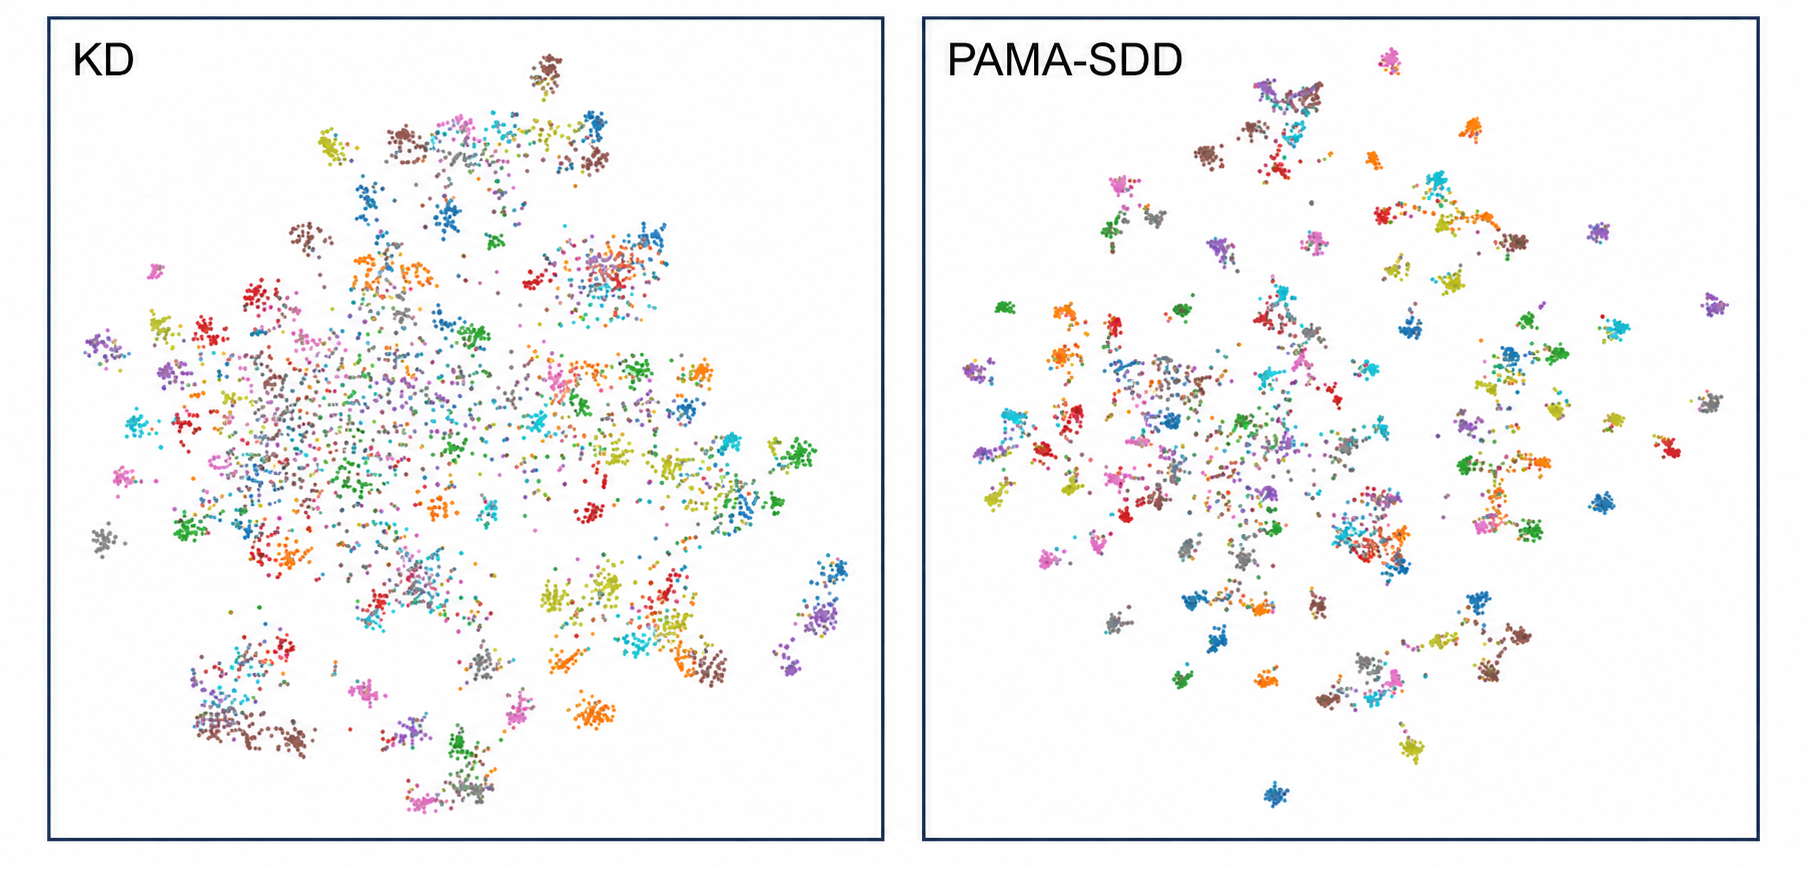
\includegraphics[width=\linewidth]{figs/t-SNE.png}
    \caption{t-SNE visualization of student features trained by KD and PAMA-SDD++. Compared with KD, PAMA-SDD++ produces more compact intra-class distributions and clearer inter-class separation.}
    \label{fig:tsne_visualization}
\end{figure}

The KD-distilled student forms several preliminary clusters, but the overall
distribution still shows noticeable inter-class overlap. Some semantically
similar categories are mixed in the feature space, and samples from the same
class are relatively scattered. This suggests that global-output supervision
can transfer class-discriminative knowledge, but it does not sufficiently
regularize the multi-scale semantic structure of the student representation.

By contrast, the student trained with PAMA-SDD++ exhibits more compact
intra-class distributions and clearer inter-class margins. The improvement
is especially visible for visually similar or background-complex categories,
where feature mixing is reduced. This visualization is consistent with the
design of PAMA-SDD++: PSPC provides a semantically coherent multi-scale
feature basis, CSAM introduces cross-scale agent-mediated context, RA-PAMA
reduces unreliable local supervision, and relation-graph GAC aligns the
teacher and student semantic structures. Therefore, the t-SNE results
qualitatively support that PAMA-SDD++ improves student feature
representation by jointly enhancing local discrimination and global semantic
consistency.

\subsubsection{Attention Visualization}

To further analyze the effect of global semantic mediation, we visualize
the attention responses of students distilled by SDD and PAMA-SDD++ on
CUB-200-2011. As shown in Figure~\ref{fig:attention_visualization}, the
SDD-distilled student can focus on some discriminative regions, but its
responses are more fragmented and may be biased toward isolated
high-contrast parts or background textures. This observation is
consistent with the limitation of fixed grid-based local supervision.

By contrast, the PAMA-SDD++-distilled student produces more coherent
responses over the target object. The highlighted regions cover the
bird's discriminative parts more continuously while suppressing
irrelevant background responses. This result suggests that CSAM helps local
regions exchange global contextual information through cross-scale agent
tokens, while LGC and relation-graph GAC encourage the student to inherit the
teacher's global semantic organization. The visualization therefore provides
qualitative evidence that PAMA-SDD++ improves the balance between local
discrimination and global consistency.

\begin{figure}[pos=t]
    \centering
    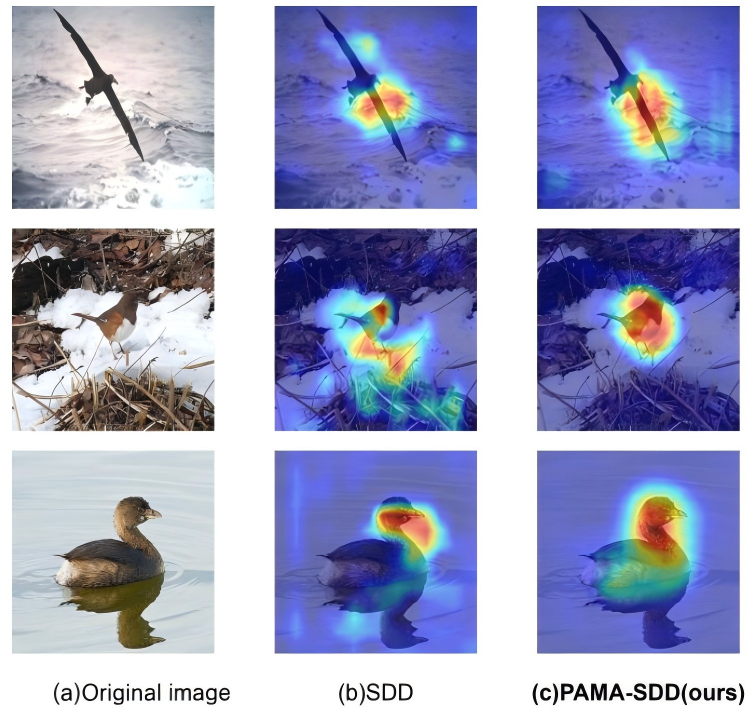
\includegraphics[width=\linewidth]{figs/attention_visualization1.png}
    \caption{Attention visualization of student models distilled by SDD and PAMA-SDD++ on CUB-200-2011. PAMA-SDD++ produces more coherent object-level responses while preserving discriminative local regions.}
    \label{fig:attention_visualization}
\end{figure}

%\subsection{Complexity and Inference Cost}
%\label{subsec:complexity_experiment}
%
%PAMA-SDD++ introduces PSPC, CSAM, local-logit construction, LGC, and GAC alignment
%only during training. These components are used to construct richer
%supervision signals and to guide the optimization of the student. They are
%not retained for deployment. Therefore, the inference-time parameter number,
%FLOPs, and latency are identical to those of the original student network.
%This property is important for practical model compression because the
%proposed method improves training supervision without increasing the cost of
%the final deployed model.
%
%From the training perspective, PSPC performs lightweight channel projection
%and adjacent-scale fusion, while CSAM replaces dense region-to-region attention
%with pixel--agent--pixel interaction. Since the number of agent tokens is
%much smaller than the number of spatial tokens, the CSAM cost grows
%approximately linearly with the spatial token number for a fixed agent grid.
%This makes the proposed framework more suitable for multi-scale
%distillation than standard self-attention.

\subsection{Discussion}
\label{subsec:discussion}

The results support three observations. First, the gains are not tied to a
particular logit objective: PAMA-SDD++ improves KD-, DKD-, and NKD-based SDD
across CIFAR-100, ImageNet-1K, and CUB-200-2011. This suggests that the
proposed mediation is an orthogonal improvement to local-logit distillation,
rather than another specialized logit loss. Second, the ablations separate the
roles of the components. PSPC improves the feature basis on which local logits
are built, CSAM returns global context to local regions, RA-PAMA reduces the
effect of unreliable teacher partitions, and LGC/GAC constrain local
predictions and agent relations to remain consistent with the teacher's global
semantics. Third, the largest improvements appear on CUB-200-2011, where the
student must use subtle local parts without losing object-level identity. This
is precisely the regime in which independent grid supervision is most likely
to fragment.

The broader implication is that local distillation should not be treated as
simply increasing the number of teacher targets. A local target is useful only
when its reliability and semantic context are controlled. PAMA-SDD++ keeps the
SDD interface but changes how the local evidence is used: regions are filtered
by teacher confidence, calibrated by a semantic pyramid, mediated by compact
agents, and regularized against global teacher belief and agent relations.
Because all of these mechanisms are used only in training, the method improves
the supervision process without changing the deployed student.

\section{Conclusion}
\label{sec:conclusion}
We presented PAMA-SDD++, a reliability-aware pyramid-agent framework for
scale-decoupled knowledge distillation. The method starts from a limitation of
grid-based local supervision: local logits expose spatial evidence, but fixed
partitions can be unreliable and semantically isolated. PAMA-SDD++ addresses
this limitation with stable frozen-teacher targets, PSPC-based pyramid
calibration, CSAM-based agent mediation, reliability-aware local
distillation, LGC, and relation-graph GAC. Across CIFAR-100, ImageNet-1K, and
CUB-200-2011, the framework improves multiple SDD baselines without increasing
student inference cost. The results indicate that the key to stronger local
distillation is not only to expose more regions, but to transfer local
evidence under reliability and global semantic constraints. Future work can
extend this principle to dense prediction tasks, including object detection
and semantic segmentation, where local evidence and global context are tightly
coupled~\cite{carion2020detr,qiao2021detectors,xie2021segformer}.
% \section{Bibliography}

% Two bibliographic style files (\verb+*.bst+) are provided ---
% {model1-num-names.bst} and {model2-names.bst} --- the first one can be
% used for the numbered scheme. This can also be used for the numbered
% with new options of {natbib.sty}. The second one is for the author year
% scheme. When  you use model2-names.bst, the citation commands will be
% like \verb+\citep+,  \verb+\citet+, \verb+\citealt+ etc. However when
% you use model1-num-names.bst, you may use only \verb+\cite+ command.

% \verb+thebibliography+ environment.  Each reference is a\linebreak
% \verb+\bibitem+ and each \verb+\bibitem+ is identified by a label,
% by which it can be cited in the text:

% \noindent In connection with cross-referencing and
% possible future hyperlinking it is not a good idea to collect
% more that one literature item in one \verb+\bibitem+.  The
% so-called Harvard or author-year style of referencing is enabled
% by the \LaTeX{} package {natbib}. With this package the
% literature can be cited as follows:

% \begin{enumerate}[\textbullet]
% \item Parenthetical: \verb+\citep{WB96}+ produces (Wettig \& Brown, 1996).
% \item Textual: \verb+\citet{ESG96}+ produces Elson et al. (1996).
% \item An affix and part of a reference:\break
% \verb+\citep[e.g.][Ch. 2]{Gea97}+ produces (e.g. Governato et
% al., 1997, Ch. 2).
% \end{enumerate}

% In the numbered scheme of citation, \verb+\cite{<label>}+ is used,
% since \verb+\citep+ or \verb+\citet+ has no relevance in the numbered
% scheme.  {natbib} package is loaded by {cas-dc} with
% \verb+numbers+ as default option.  You can change this to author-year
% or harvard scheme by adding option \verb+authoryear+ in the class
% loading command.  If you want to use more options of the {natbib}
% package, you can do so with the \verb+\biboptions+ command.  For
% details of various options of the {natbib} package, please take a
% look at the {natbib} documentation, which is part of any standard
% \LaTeX{} installation.

% \appendix
% \section{My Appendix}
% Appendix sections are coded under \verb+\appendix+.

% \verb+\printcredits+ command is used after appendix sections to list 
% author credit taxonomy contribution roles tagged using \verb+\credit+ 
% in frontmatter.

% \printcredits

%% Loading bibliography style file
\bibliographystyle{model1-num-names}
%\bibliographystyle{cas-model2-names}

% Loading bibliography database
\bibliography{cas-refs}


%\vskip3pt

% \bio{}
% Author biography without author photo.
% Author biography. Author biography. Author biography.
% Author biography. Author biography. Author biography.
% Author biography. Author biography. Author biography.
% Author biography. Author biography. Author biography.
% Author biography. Author biography. Author biography.
% Author biography. Author biography. Author biography.
% Author biography. Author biography. Author biography.
% Author biography. Author biography. Author biography.
% Author biography. Author biography. Author biography.
% \endbio

% \bio{figs/pic1}
% Author biography with author photo.
% Author biography. Author biography. Author biography.
% Author biography. Author biography. Author biography.
% Author biography. Author biography. Author biography.
% Author biography. Author biography. Author biography.
% Author biography. Author biography. Author biography.
% Author biography. Author biography. Author biography.
% Author biography. Author biography. Author biography.
% Author biography. Author biography. Author biography.
% Author biography. Author biography. Author biography.
% \endbio

% \bio{figs/pic1}
% Author biography with author photo.
% Author biography. Author biography. Author biography.
% Author biography. Author biography. Author biography.
% Author biography. Author biography. Author biography.
% Author biography. Author biography. Author biography.
% \endbio

\end{document}

